%
% Copyright 2018 Joel Feldman, Andrew Rechnitzer and Elyse Yeager.
% This work is licensed under a Creative Commons Attribution-NonCommercial-ShareAlike 4.0 International License.
% https://creativecommons.org/licenses/by-nc-sa/4.0/
%
\questionheader{ex:s3.2}
%%%%%%%%%%%%%%%%%%
\subsection*{\Conceptual}
%%%%%%%%%%%%%%%%%%


\begin{Mquestion}
Suppose the quantities $P$ and $Q$ are related by the formula $P=Q^3$. $P$ and $Q$ are changing with respect to time, $t$. Given this information, which of the following are problems you could solve?
\begin{enumerate}[i.]
\item Given $\ds\diff{P}{t}(0)$, find $\ds\diff{Q}{t}(0)$. (Remember: the notation $\ds\diff{P}{t}(0)$ means the derivative of $P$ with respect to $t$ at the time $t=0$.)
\item Given $\ds\diff{P}{t}(0)$ and the value of $Q$ when $t=0$, find $\ds\diff{Q}{t}(0)$.
\item Given $\ds\diff{Q}{t}(0)$, find $\ds\diff{P}{t}(0)$.
\item Given $\ds\diff{Q}{t}(0)$  and the value of $P$ when $t=0$, find $\ds\diff{P}{t}(0)$.
\end{enumerate}
\end{Mquestion}
\begin{hint}
If you know $P$, you can figure out $Q$.
\end{hint}
\begin{answer}
ii and iv
\end{answer}
\begin{solution}
We have an equation relating $P$ and $Q$:
\begin{align*}
P&=Q^3
\intertext{We differentiate implicitly with respect to a third variable, $t$:}
\diff{P}{t}&=3Q^2\cdot\diff{Q}{t}
\end{align*}
If we know two of the three quantities $\ds\diff{P}{t}$, $Q$, and $\ds\diff{Q}{t}$, then we can find the third. Therefore, ii is a question we can solve. If we know $P$, then we also know $Q$ (it's just the cube root of $P$), so also we can solve iv. However, if we know neither $P$ nor $Q$, then we can't find $\ds\diff{P}{t}$ based only off $\ds\diff{Q}{t}$, and
we can't find $\ds\diff{Q}{t}$ based only off $\ds\diff{P}{t}$. So we can't solve i or iii.
\end{solution}




%%%%%%%%%%%%%%%%%%
\subsection*{\Procedural}
%%%%%%%%%%%%%%%%%%

%%%%%%%%%%%%%%%%%%
%\subsubsection*{Problems in which the relationship between variables is expressly given}
%%%%%%%%%%%%%%%%%%
\Instructions{For problems \ref{s3.2relationshipfirst} through
\ref{s3.2relationshiplast}, the relationship between several variables is explicitly given. Use this information to relate their rates of change.}

\begin{Mquestion}[2007H]\label{s3.2relationshipfirst}
 A point is moving on the unit circle
$\set{ (x, y)~:~ x^2 + y^2 = 1 }$ in the $xy$--plane.
At $(2/\sqrt{5}, 1/\sqrt{5})$, its $y$--coordinate is increasing at rate 3.
What is the rate of change of its $x$--coordinate?
\end{Mquestion}
\begin{hint}
Since the point moves along the unit circle, we know that $x^2+y^2=1$, where $x$ and $y$ are functions of time.
\end{hint}
\begin{answer}
$-\dfrac{3}{2}$
\end{answer}
\begin{solution}
 Suppose that at time $t$, the point is at $\big(x(t),y(t)\big)$.
Then $x(t)^2+y(t)^2=1$ so that $2x(t)x'(t)+2y(t)y'(t)=0$. We are told that
at some time $t_0$, $x(t_0)=2/\sqrt{5}$, $y(t_0)=1/\sqrt{5}$ and $y'(t_0)=3$.
Then
\begin{align*}
2x(t_0)x'(t_0)+2y(t_0)y'(t_0)&=0 \qquad \Rightarrow\\
2\left(\frac{2}{\sqrt{5}}\right)x'(t)+2\left(\frac{1}{\sqrt5}\right)(3)&=0
\qquad \Rightarrow\\
x'(t_0)&=-\frac{3}{2}
\end{align*}
\end{solution}


\begin{question}[1997D, 2012H]
The quantities $P,\ Q$ and $R$ are functions of time and are related
by the equation $R=PQ$. Assume that $P$ is increasing instantaneously at
the rate of $8\%$ per year and that $Q$ is decreasing instantaneously at
the rate of $2\%$ per year. That is, $\dfrac{P'}{P}=0.08$ and $\dfrac{Q'}{Q}=-0.02$.
Determine the percentage rate of change for $R$.
\end{question}
\begin{hint}
You'll need some implicit differentiation: what should your variable be?
Example~\ref*{eg:percentGrowth} shows how to work with percentage rate of change.
\end{hint}
\begin{answer} $6\%$
\end{answer}
\begin{solution}
The instantaneous percentage rate of change for $R$ is
\begin{align*}
100\frac{R'}{R}&=100\frac{(PQ)'}{PQ}&\mbox{R=PQ}\\
&=100\frac{P'Q+PQ'}{PQ}&\mbox{product rule}\\
&=100\left[\frac{P'}{P}+\frac{Q'}{Q}\right]&\mbox{simplify}\\
&=100[0.08-0.02]
=6\%
\end{align*}
\end{solution}


\begin{question}[1997A]\label{s3.2relationshiplast}
Three quantities, $F$, $P$ and $Q$ all depend upon time
$t$ and are related by the equation
$$
F=\frac{P}{Q}
$$
\begin{enumerate}[(a)]
\item\label{s3.2FPQ1} Assume that at a particular moment in time $P=25$ and $P$
is increasing at the instantaneous rate of 5 units/min. At the same moment,
$Q=5$ and $Q$ is increasing at the instantaneous rate of 1 unit/min. What
is the instantaneous rate of change in $F$ at this moment?
\item\label{s3.2FPQ2} Assume that at another moment in time $P$ is increasing at
the instantaneous rate of $10\%$ and $Q$ is decreasing at the instantaneous
rate $5\%$. What can you conclude about the rate of change of $F$ at this
moment?
\end{enumerate}
\end{question}
\begin{hint} For \eqref{s3.2FPQ2}, refer to Example~\ref*{eg:percentGrowth} for percentage rate of change.
\end{hint}
\begin{answer}
\eqref{s3.2FPQ1} 0\qquad
\eqref{s3.2FPQ2} $100\dfrac{F'}{F}=15\%$, or $F'=0.15F$
\end{answer}
\begin{solution}
\eqref{s3.2FPQ1}
By the quotient rule, $F'=\dfrac{P'Q-PQ'}{Q^2}$. At the moment in question,
$F'=\dfrac{5\times5-25\times 1}{5^2}=0.$

\eqref{s3.2FPQ2}
We are told that, at the second moment in time,
$P'=0.1 P$  and $Q'=-0.05 Q$

 $\big($or equivalently $100\frac{P'}{P}=10$ and $100\frac{Q'}{Q}=-5\big)$. Substituting in these values:

\begin{align*}
F'&=\frac{P'Q-PQ'}{Q^2}\\
&=\frac{0.1PQ-P(-0.05Q)}{Q^2}\\
&=\frac{0.15PQ}{Q^2}\\
&=0.15\frac{P}{Q}\\
&=0.15 F\qquad
\implies\\
 F'&=0.15F\end{align*}

 or  $100\frac{F'}{F}=15\%$. That is, the instantaneous percentage rate of change of $F$ is 15\%.
\end{solution}





%%%%%%%%%%%%%%%%%%
%\subsubsection*{Problems involving the Pythagorean Theorem}
%%%%%%%%%%%%%%%%%%
\Instructions{For Questions \ref{s3.2Pythagorusfirst} through
\ref{s3.2Pythagoruslast}, look for a way to use the Pythagorean Theorem.}

\begin{question}[2015Q]\label{s3.2Pythagorusfirst}
Two particles move in the Cartesian plane. Particle A travels on the $x$-axis
starting at  $(10,0)$ and moving towards the origin with a speed of $2$ units
per second. Particle B travels on the $y$-axis starting at $(0,12)$ and moving
towards the origin with a speed of $3$ units per second. What is the rate of
change of the distance between the two particles when particle A reaches the
point $(4,0)$?
\end{question}
\begin{hint} Pay attention to direction, and what it means for the sign (plus/minus) of the velocities of the particles.
\end{hint}
\begin{answer}
$-\dfrac{17}{5}$ units per second
\end{answer}
\begin{solution}
\begin{itemize}
 \item The distance $z(t)$ between the particles at any moment in time is
\begin{align*}
z^2(t)&= x(t)^2+y(t)^2,
\end{align*}
where $x(t)$ is the position on the $x$-axis of the particle A at time $t$
(measured in seconds) and $y(t)$ is the position on the $y$-axis of the particle
B at the same time $t$.
\item We differentiate the above equation with respect to $t$ and get
\begin{align*}
2z \cdot z' &= 2x \cdot x' + 2 y \cdot y',
\end{align*}
\item We are told that $x'=-2$ and $y'=-3$. (The values are negative because $x$ and $y$ are decreasing.) It will take $3$ seconds
for particle $A$ to reach $x=4$, and in this time particle $B$ will reach
$y=3$.

\item At this point $z = \sqrt{x^2+y^2}=\sqrt{3^2+4^2}=5$.
\item Hence
\begin{align*}
  10z' &= 8\cdot(-2)+6\cdot(-3) = -34 \\
  z' &= -\frac{34}{10} = -\frac{17}{5} \text{ units per second}.
\end{align*}
\end{itemize}
\end{solution}



\begin{question}[2015Q]
Two particles $A$ and $B$ are placed on the Cartesian plane at $(0,0)$ and $(3,0)$
respectively. At time 0, both start to move in the $+y$ direction. Particle $A$ moves at
3 units per second, while $B$ moves at $2$ units per second. How fast is the distance
between the particles changing when particle $A$ is at a distance of $5$ units from $B$.
\end{question}
\begin{hint} You'll want to think about the difference in the $y$-coordinates of the two particles.
\end{hint}
\begin{answer} $\dfrac{4}{5}$ units per second
\end{answer}
\begin{solution}
\begin{itemize}
 \item We compute the distance $z(t)$ between the two particles after $t$ seconds as
\begin{align*}
z^2(t)&= 3^2 + (y_A(t)-y_B(t))^2,
\end{align*}
where $y_A(t)$ and $y_B(t)$ are the $y$-coordinates of particles $A$ and $B$ after $t$
seconds, and the horizontal distance between the two particles is always 3 units.
\item We are told the distance between the particles is 5 units, this happens when
\begin{align*}
  (y_A-y_B)^2 &= 5^2-3^2 = 16\\
  y_A-y_B&=4
\end{align*}
That is, when the difference in $y$-coordinates is $4$. This happens when $t=4$.

\item We differentiate the distance equation (from the first bullet point) with respect to $t$ and get
\begin{align*}
2z \cdot z' &= 2 ({y_A}' - {y_B}') (y_A - y_B),
\end{align*}
\item We know that $(y_A-y_B)=4$, and we are told that $z=5$, $y_A'=3$, and $y_B'=2$. Hence
\begin{align*}
  10z'(4) &=  2 \times1\times4 = 8
\end{align*}
\item Therefore
\begin{align*}
  z'(4) &= \frac{8}{10} = \frac{4}{5} \text{ units per second}.
\end{align*}
\end{itemize}
\end{solution}




\begin{Mquestion}[1997D]
Ship A is 400 miles directly south of Hawaii and is sailing
south at 20 miles/hour. Ship B is 300 miles directly east of Hawaii and
is sailing west at 15 miles/hour. At what rate is the distance between
the ships changing?
\end{Mquestion}
\begin{hint} Draw a picture, and be careful about signs.
\end{hint}
\begin{answer} increasing at $7$ mph
\end{answer}
\begin{solution}
\begin{center}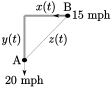
\includegraphics{ship}\end{center}

If $x(t),\ y(t)$ and $z(t)$ are the distances shown, at time
$t$, then
\begin{align*}
x(t)^2+y(t)^2&=z(t)^2
\intertext{Differentiating with respect to $t$,}
2x(t)x'(t)+2y(t)y'(t)&=2z(t)z'(t)\\
x(t)x'(t)+y(t)y'(t)&=z(t)z'(t)
\intertext{At the specified time, $x(t)$ is decreasing, so $x'(t)$ is negative.}
 (300)(-15)+(400)(20) &= \sqrt{300^2+400^2}z'(t)\\
500 z'(t)&=3500\\
z'(t)&=7 \mbox{ mph}
\end{align*}
\end{solution}


%\begin{question}[2015Q]
%Boat $A$ travels north at 30km/h and boat $B$ travels east at 40km/h. These
%boats started from the same point at 12pm. When boat $B$ has traveled 20km, how fast is the distance between boat $A$ and $B$ increasing?
%\end{question}
%\begin{answer} 16 kph
%\end{answer}
%\begin{solution}
%\begin{itemize}
% \item
%We think the start as the origin in the plane. Then, we compute the distance $z(t)$
%between boat A and B at each moment in time as
%\begin{align*}
%z^2(t)&= x(t)^2+y(t)^2,
%\end{align*}
%where $x(t)$ is the position on the $x$-axis of boat B at time $t$
%(measured in hours) and $y(t)$ is the position on the $y$-axis of boat
%A at the same time $t$.
%\item We differentiate the above equation with respect to $t$ and get
%\begin{align*}
%2z \cdot z' &= 2x \cdot x' + 2 y \cdot y',
%\end{align*}
%\item We are told that $x'=40$ and $y'=30$. Further it will take $0.5$ hours
%for boat $B$ to travel $20$km, and in this time boat $A$ will travel
%$15$km.
%\item Alternatively, write $x=40t,y=30t$ to get $t=1/2,
%x'=40,y'=30,y=15$.
%\item At this point $z = \sqrt{x^2+y^2}=\sqrt{40^2+30^2}=50$.
%\item Hence
%\begin{align*}
%  100z' &= 40\cdot(40)+30\cdot(30) = 1600 \\
%  z' &= \frac{1600}{100} =16  \text{km per hour}.
%\end{align*}
%\end{itemize}
%\end{solution}




%\begin{question}
%Child $A$ and Child $B$ are sitting in the same spot. At exactly noon, Child $A$ sees a dog, and runs due east towards it at a steady pace of 1 meter per second. One second later (at one second past noon), Child $B$ sees a spider, and runs due north away from it at a steady pace of 2 meters per second. How fast is the distance between the children increasing at three seconds past noon?
%\end{question}
%\begin{hint} Find an equation that relates the distance between the two children to each child's distance from their starting point.
%\end{hint}
%\begin{answer} $11/5$ meters per second
%\end{answer}
%\begin{solution}
%\begin{center}\begin{tikzpicture}
%\draw[thick, ->] (0,0) node[vertex]{}--(2,0) ;
%\draw (1,-.5) node{$a(t)$};
%\draw[thick, ->] (0,0)--(0,3);
%\draw (-.5,1.5) node{$b(t)$};
%\draw[dashed] (2,0) -- (0,3) node[midway, label= right:$D$]{};
%\end{tikzpicture}\end{center}
%\begin{itemize}
% \item The children start at the same point. Let $a$ be Child $A$'s distance from that point, and let $b$ be Child $B$'s distance from that point. Then we know $\diff{a}{t}=1$ meter per second, and $\diff{b}{t}=2$ meters per second.  Note these rates are both positive.
%
% \item Our units are measured in seconds. Let noon be $t=0$. If $D$ is the distance between the children, we want to know $\diff{D}{t}$ when $t=3$.
%
%\item So, we need an equation relating $a$, $b$, and $D$. Of course this equation is
%\[D^2=a^2+b^2\]
%and we differentiate with respect to $t$:
%\[2D\diff{D}{t} = 2a\diff{a}{t}+2b\diff{b}{t}\]
%
%\item To solve for $\diff{D}{t}$, we need $a$, $b$, and $D$ when $t=3$. Since Child $A$ starts running at $t=0$, $\left.a\right|_{t=3}=1\cdot 3=3$ meters. Since Child $B$ starts running at $t=1$, $\left.b\right|_{t=3}=2(3-1)=4$ meters. Then $\left.D\right|_{t=3}=\sqrt{3^2+4^2}=5$.
%
%\item Now we solve for $\diff{D}{t}$:
%\begin{align*}
%2D\diff{D}{t} &= 2a\diff{a}{t}+2b\diff{b}{t}\\
%2(5)\left.\diff{D}{t}\right|_{t=3} &=2(3)(1)+2(4)(2)\\
%\left.\diff{D}{t}\right|_{t=3}&={\frac{11}{5}} \mbox{ meters per second}
%\end{align*}
%
%\item Equivalently, we can write $a=t$ and $b=2(t-1)$, so $D^2=a^2+b^2=t^2+4(t-1)^2$. Then
%\[2D\diff{D}{t} = 2t+8(t-1)\]
%So
%\[2(5)\left.\diff{D}{t}\right|_{t=3} = 2(3)+8(3-1)=22\]
%hence $\ds\diff{D}{t}={\frac{11}{5}}$ meters per second.
%\end{itemize}
%\end{solution}



\begin{Mquestion}[2015Q]
Two tall sticks are vertically planted into the ground, separated by a distance of $30$ cm. We simultaneously put two snails at the base of each stick. The two snails then begin to climb their respective sticks. The first snail is moving with a speed of $25$ cm per minute, while the second snail is moving with a speed of $15$ cm per minute.
What is the rate of
change of the distance between the two snails when the first snail reaches $100$ cm above the ground?
\end{Mquestion}
\begin{hint}
You'll want to think about the \emph{difference} in height of the two snails.
\end{hint}
\begin{answer}
$8$ cm per minute
\end{answer}
\begin{solution}
\begin{itemize}
 \item
We compute the distance $d(t)$ between the two snails after $t$ minutes as
\begin{align*}
d^2(t)&= 30^2 + (y_1(t)-y_2(t))^2,
\end{align*}
where $y_1(t)$ is the altitude of the first snail, and $y_2(t)$ the altitude of the second snail after $t$ minutes.
\item We differentiate the above equation with respect to $t$ and get
\begin{align*}
2d \cdot d' &= 2 ({y_1}' - {y_2}') (y_1 - y_2)\\
d \cdot d' &=  ({y_1}' - {y_2}') (y_1 - y_2)
\end{align*}
\item We are told that ${y_1}'=25$ and ${y_2}'=15$. It will take $4$ minutes
for the first snail to reach $y_1=100$, and in this time  the second snail will reach
$y_2=60$.
\item At this point $d^2 = 30^2 + (100-60)^2 = 900 + 1600 = 2500$, hence $d = 50$.
\item Therefore
\begin{align*}
50  d' &=  (25 - 15) \times (100 - 60)   \\
  d' &= \frac{400}{50} = 8 \text{ cm per minute}.
\end{align*}
\end{itemize}
\end{solution}



\begin{question}[2015Q]\label{s3.2Pythagoruslast}
A $20$m long extension ladder leaning against a wall starts collapsing in on itself at a
rate of $2$m/s, while the foot of the ladder remains a constant $5$m from the wall.
How fast is the ladder moving down the wall after $3.5$ seconds?
\end{question}
\begin{hint} The length of the ladder is changing.
\end{hint}
\begin{answer}
$-\dfrac{13}{6}$ metres per second
\end{answer}
\begin{solution}
\begin{itemize}
 \item
    If we write $z(t)$ for the length of the ladder at time $t$ and $y(t)$ for the height of the top end of the ladder at time $t$ we have
    \[
        z(t)^2 = 5^2 + y(t)^2.
    \]
\item We differentiate the above equation with respect to $t$ and get
\begin{align*}
2z \cdot z' &= 2y \cdot y',
\end{align*}
\item We are told that $z'(t)=-2$, so $z(3.5)=20-3.5\cdot2 = 13$.
\item At this point $y = \sqrt{z^2-5^2} = \sqrt{169-25} = \sqrt{144} = 12$.
\item Hence
\begin{align*}
  2\cdot 13 \cdot (-2) &= 2 \cdot 12 y' \\
  y' &= -\frac{2\cdot 13}{12} = -\frac{13}{6} \text{ meters per second}.
\end{align*}
\end{itemize}
\end{solution}



%%%%%%%%%%%%%%%%%%
%\subsubsection*{Problems involving similar triangles and other trigonometric tidbits}
%%%%%%%%%%%%%%%%%%
\Instructions{
For Questions \ref{s3.2trianglesfirst} through
\ref{s3.2triangleslast}, look for tricks from trigonometry.}


\begin{Mquestion}\label{s3.2trianglesfirst}
A watering trough has a cross section shaped like an isosceles trapezoid. The trough is 2 metres long, 50 cm high, 1 metre wide at the top, and 60 cm wide at the bottom.
\begin{center}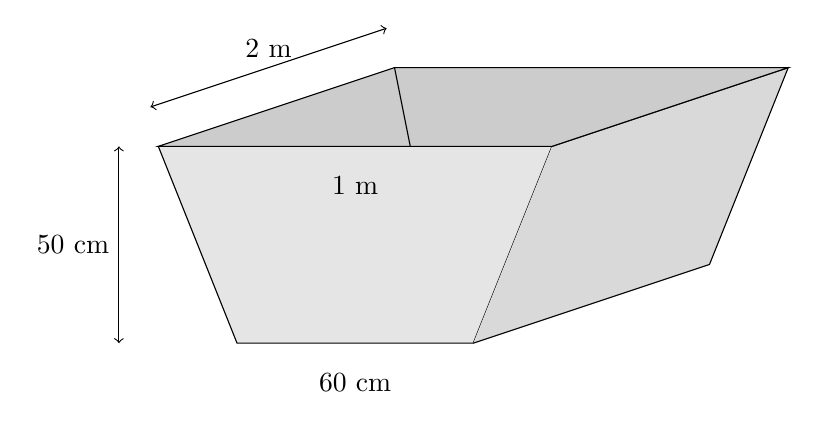
\begin{tikzpicture}
\draw[fill=black!10] (0,0)--(3,0)--(4,2.5)--(-1,2.5)--cycle;
\draw[fill=black!15] (4,2.5)--(7,3.5)--(6,1)--(3,0);
\draw[fill=black!20] (-1,2.5)--(2,3.5)--(7,3.5)--(4,2.5)--cycle;
\draw (2,3.5)--(2.2,2.5);
\draw (1.5,-.5) node{$60$ cm};
\draw (1.5,2) node{$1$ m};
\draw[<->] (-1.5,0)--(-1.5,2.5) node[midway, left]{$50$ cm};
\draw[<->] (-1.1,3)--(1.9,4) node[midway, above]{$2$ m};
\end{tikzpicture}\end{center}
A pig is drinking water from the trough at a rate of 3 litres per minute. When the height of the water is 25 cm, how fast is the height decreasing?
\end{Mquestion}
\begin{hint}
If a  trapezoid has height $h$ and (parallel) bases $b_1$ and $b_2$, then its area is $h\left(\frac{b_1+b_2}{2}\right)$. To figure out how wide the top of the water is when the water is at height $h$, you can cut the trapezoid up into a rectangle and two triangles, and make use of similar triangles.
\end{hint}
\begin{answer} The height of the water is decreasing at
$\dfrac{3}{16}=0.1875~\frac{\mathrm{cm}}{\mathrm{min}}$.
\end{answer}
\begin{solution}
What we're given is $\ds\diff{V}{t}$ (where $V$ is volume of water in the trough, and $t$ is time), and what we are asked for is $\ds\diff{h}{t}$ (where $h$ is the height of the water). So, we need an equation relating $V$ and $h$. First, let's get everything in the same units: centimetres.

\begin{center}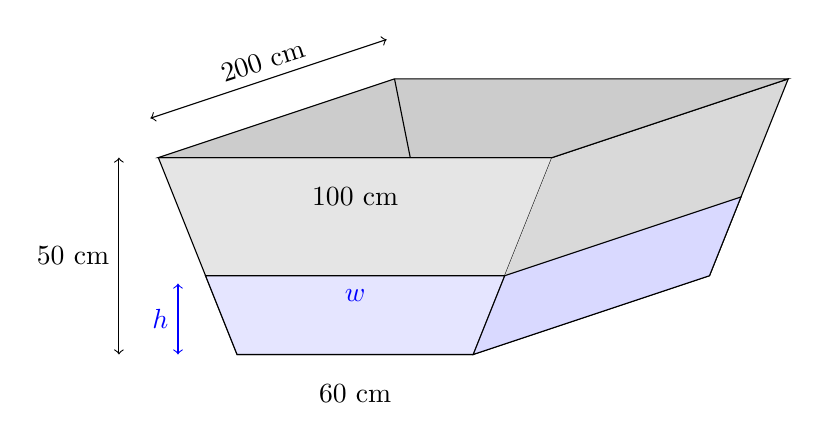
\begin{tikzpicture}
\draw[fill=black!10] (0,0)--(3,0)--(4,2.5)--(-1,2.5)--cycle;
\draw[fill=black!15] (4,2.5)--(7,3.5)--(6,1)--(3,0);
\draw[fill=black!20] (-1,2.5)--(2,3.5)--(7,3.5)--(4,2.5)--cycle;
\draw (2,3.5)--(2.2,2.5);
\draw (1.5,-.5) node{$60$ cm};
\draw (1.5,2) node{$100$ cm};
\draw[<->] (-1.5,0)--(-1.5,2.5) node[midway, left]{$50$ cm};
\draw[<->] (-1.1,3)--(1.9,4) node[midway, above, rotate=18]{$200$ cm};
\draw[fill=blue!10] (0,0)--(3,0)--(3.4,1)--(-.4,1)--cycle;
\draw[fill=blue!15](3,0)--(6,1)--(6.4,2)--(3.4,1)--cycle;
\draw[<->, blue] (-.75,0)--(-.75,.9) node[midway, left]{$h$};
\draw[blue] (1.5,.75)node{$w$};
\end{tikzpicture}\end{center}

We can calculate the volume of water in the trough by multiplying the area of its trapezoidal cross section by 200 cm. A  trapezoid with height $h$ and bases $b_1$ and $b_2$ has area $h\left(\frac{b_1+b_2}{2}\right)$. (To see why this is so, draw the trapezoid as a rectangle flanked by two triangles.)
So, using  $w$ as the width of the top of the water (as in the diagram above), the area of the cross section of the water in the trough is
\[A=h\left(\frac{60+w}{2}\right)\]
and therefore the volume of water in the trough is
\[V=100h(60+w)~\text{cm}^3.\]
We need a formula for $w$ in terms of $h$.
If we draw lines straight up from the bottom corners of the trapezoid, we break it into rectangles and triangles.
\begin{center}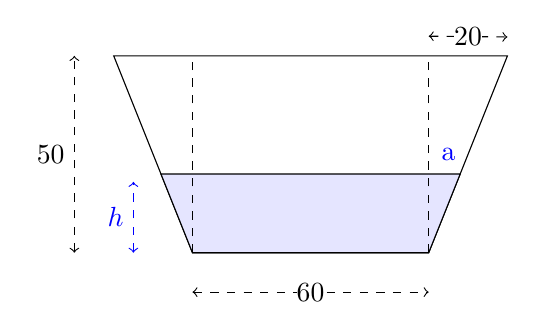
\begin{tikzpicture}
\draw (0,0)--(3,0)--(4,2.5)--(-1,2.5)--cycle;
\draw[<->, dashed] (0,-.5)--(3,-.5) node[midway, shape=rectangle, fill=white, inner sep=0]{$60$ };
%\draw[<->, dashed, blue] (-.5,1.5)--(3.5,1.5) node[midway, shape=rectangle, fill=white, inner sep=0]{$w$ };
%\draw[<->, dashed](-1,3)-- (4,3) node[midway, shape=rectangle, fill=white, inner sep=0]{$100$ };
\draw[<->, dashed] (-1.5,0)--(-1.5,2.5) node[midway, left]{$50$ };
\draw[fill=blue!10] (0,0)--(3,0)--(3.4,1)--(-.4,1)--cycle;
\draw[<->, blue, dashed] (-.75,0)--(-.75,.9) node[midway, left]{$h$};
\draw[dashed] (0,0)--(0,2.5) (3,0)--(3,2.5);
\draw[blue] (3.25,1.25) node{a};
\draw[<->, dashed] (3,2.75) --(4,2.74)node[midway, shape=rectangle, fill=white, inner sep=0]{$20$};
\end{tikzpicture}\end{center}
 Using similar triangles,
$\dfrac{a}{h}=\dfrac{20}{50}$,
so $a=\dfrac{2}{5}h$. Then
\begin{align*}
w&=60+2a\\&=60+2\left(\frac{2}{5}h\right)=60+\frac{4}{5}h
\intertext{so}
V&=100h(60+w)\\&=100h(120+\frac{4}{5}h)\\&=80h^2+12000h
\intertext{This is the equation we need, relating $V$ and $h$. Differentiating implicitly with respect to $t$:}
\diff{V}{t}
&=2\cdot80h\cdot\diff{h}{t}+12000\diff{h}{t}\\
&=\left(160h+12000\right)\diff{h}{t}
\intertext{We are given that $h=25$ and $\ds\diff{V}{t}=3$ litres per minute. Converting to cubic centimetres, $\ds\diff{V}{t} = -3000$ cubic centimetres per minute. So:}
-3000&=\left(160\cdot25+12000\right)\diff{h}{t}\\
\diff{h}{t}&=-\frac{3}{16}=-.1875~\frac{\mathrm{cm}}{\mathrm{min}}
\end{align*}
So, the water level is dropping at $\dfrac{3}{16}$ centimetres per minute.
\end{solution}





\begin{question}
A tank is 5 metres long, and has a trapezoidal cross section with the dimensions shown below.

\begin{center}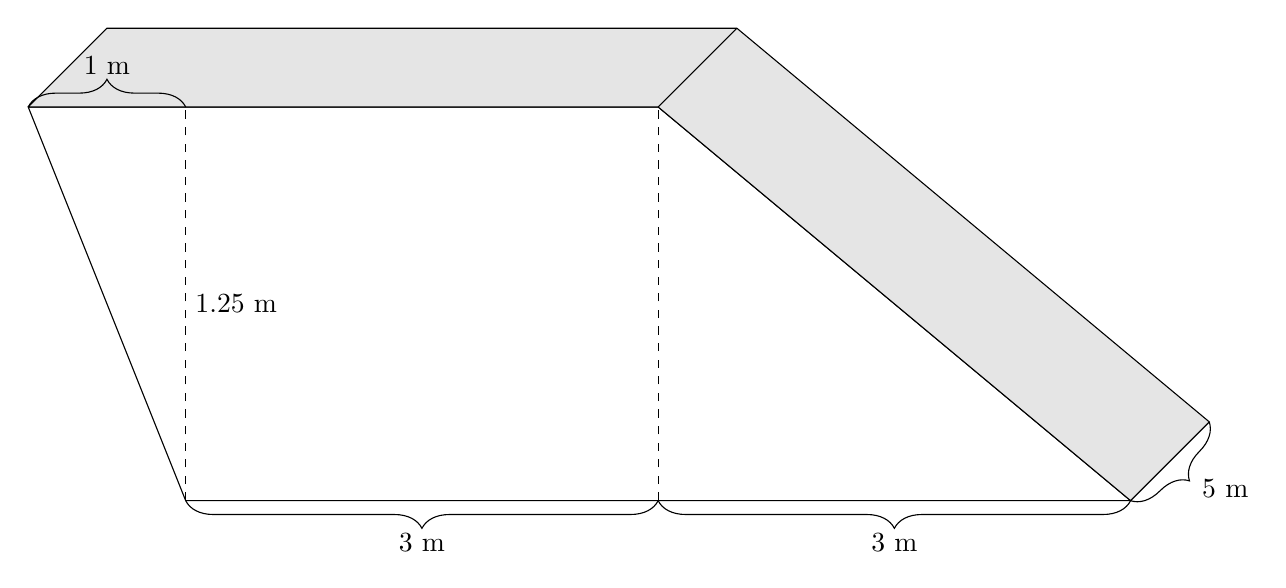
\begin{tikzpicture}
\draw (0,0)--(12,0)--(6,5)--(-2,5)--cycle;
\draw[fill=gray!20] (-2,5)--(-1,6)--(7,6)--(13,1)--(12,0)--(6,5)--(-2,5);
\draw (6,5)--(7,6);
\draw[dashed] (0,0)--(0,5) node[midway, right]{$1.25$ m};
\draw[dashed] (6,0)--(6,5);
\draw[decorate, decoration={brace, amplitude=10pt, mirror}] (6,0)--(12,0) node[midway, yshift=-15pt]{3 m};
\draw[decorate, decoration={brace, amplitude=10pt, mirror}] (0,0)--(6,0) node[midway, yshift=-15pt]{3 m};
\draw[decorate, decoration={brace, amplitude=10pt}] (-2,5)--(0,5) node[midway, yshift=15pt]{1 m};
\draw[decorate, decoration={brace, amplitude=10pt, mirror}] (12,0)--(13,1) node[midway, xshift=20pt, yshift=-10 pt]{5 m};
\end{tikzpicture}
\end{center}
A hose is filling the tank up at a rate of one litre per second. How fast is the height of the water increasing when the water is 10 centimetres deep?
\end{question}

\begin{hint}
Be careful with units. One litre is 1000 cm$^3$, which is not the same as $10$ m$^3$.
\end{hint}

\begin{answer}
$\dfrac{1}{29200}$ metres per second (or about 1 centimetre every five minutes)
\end{answer}

\begin{solution}
If $V$ is the volume of the water in the tank, and $t$ is time, then we are given $\ds\diff{V}{t}$. What we want to know is $\ds\diff{h}{t}$, where $h$ is the height of the water in the tank. A reasonable plan is to find an equation relating $V$ and $h$, and differentiate it implicitly with respect to $t$.

Let's be a little careful about units.
The volume of water in the tank is
\[\text{(area of cross section of water)$\times$(length of tank)}\] If we measure these values in metres (area in square metres, length in metres), then the volume is going to be in cubic metres. So, when we differentiate with respect to time, our units will be cubic metres per second. The water is flowing in at one litre per second, or $1000$ cubic centimetres per second. So, we either have to measure our areas and distances in centimetres, or convert litres to cubic metres. We'll do the latter, but both are fine.

 If we imagine one cubic metre as a cube, with each side of length 1 metre, then it's easy to see the volume inside is $(100)^3=10^6$ cubic centimetres: it's the volume of a cube with each side of length 100 cm. Since a litre is $10^3$ cubic centimetres, and a cubic metre is $10^{6}$ cubic centimetres, one litre is $10^{-3}$ cubic metres.
So, \textcolor{red}{$\ds\diff{V}{t}=\frac{1}{10^3}$} cubic metres per second.

Let $h$ be the height of the water (in metres). We can figure out the area of the cross section by breaking it into three pieces: a triangle on the left, a rectangle in the middle, and a trapezoid on the right.

\begin{center}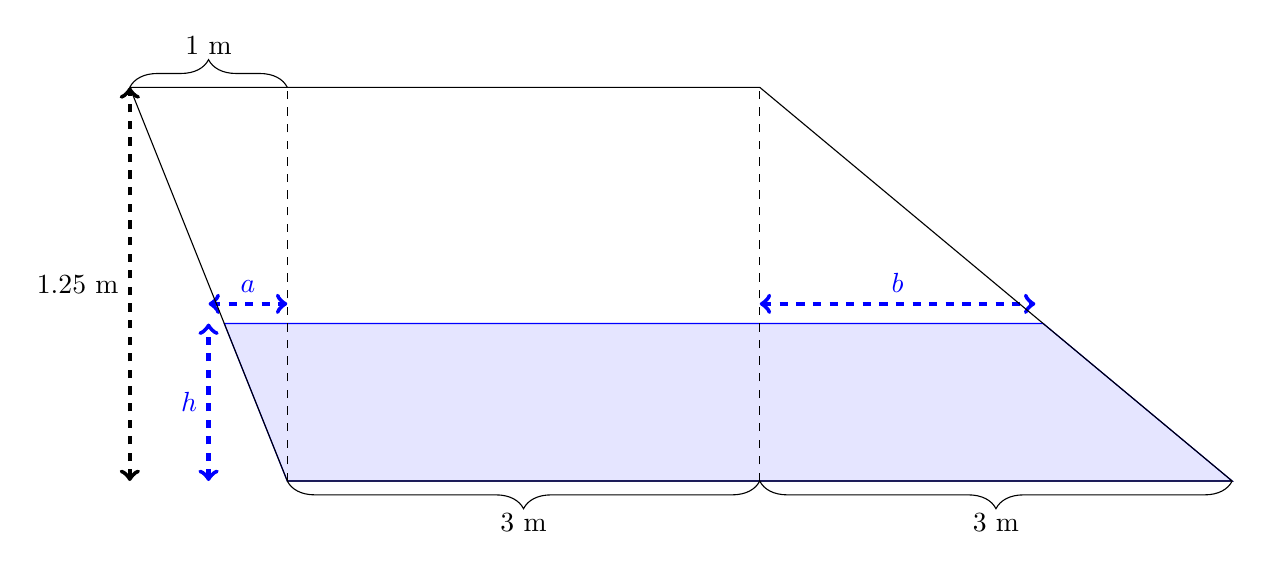
\begin{tikzpicture}
\draw[blue, fill=blue!10] (-.8,2)--(9.6,2)--(12,0)--(0,0)--cycle;
\draw[blue, dashed, <->, ultra thick] (-1,0)--(-1,2) node[midway, left]{$h$};
\draw[blue, dashed, <->, ultra thick] (-1,2.25)--(0,2.25) node[midway, above]{$a$};
\draw[blue, dashed, <->, ultra thick] (6.,2.25)--(9.5,2.25) node[midway, above]{$b$};
\draw (0,0)--(12,0)--(6,5)--(-2,5)--cycle;
\draw[dashed] (0,0)--(0,5);
\draw[dashed, <->, ultra thick] (-2,0)--(-2,5) node[midway, left]{$1.25$ m};
\draw[dashed] (6,0)--(6,5);
\draw[decorate, decoration={brace, amplitude=10pt, mirror}] (6,0)--(12,0) node[midway, yshift=-15pt]{3 m};
\draw[decorate, decoration={brace, amplitude=10pt, mirror}] (0,0)--(6,0) node[midway, yshift=-15pt]{3 m};
\draw[decorate, decoration={brace, amplitude=10pt}] (-2,5)--(0,5) node[midway, yshift=15pt]{1 m};
\end{tikzpicture}
\end{center}

\begin{itemize}
\item The triangle on the left has height $h$ metres. Let its base be $a$ metres.
It forms a similar triangle with the triangle whose height is 1.25 metres and width is 1 metre, so:
\begin{align*}
\frac{a}{h}&=\frac{1}{1.25}\\
a&=\frac{4}{5}h
\intertext{So, the area of the triangle on the left is}
\frac{1}{2}ah&=\frac{2}{5}h^2
\end{align*}

\item The rectangle in the middle has length 3 metres and height $h$ metres, so its area is $3h$ square metres.

\item The trapezoid on the right is a portion of a triangle with base 3 metres and height 1.25 metres. So, its area is
\begin{align*}&~\underbrace{\left(\frac{1}{2}(3)(1.25)\right) }_{\mbox{area of big triangle}}- \underbrace{\left(\frac{1}{2}(b)(1.25-h)\right)}_{\mbox{area of little triangle}}
\intertext{The little triangle (of base $b$ and height $1.25-h$) is formed by the \emph{air} on the right side of the tank. It is a similar triangle to the triangle of base 3 and height 1.25, so}
\frac{b}{1.25-h}&=\frac{3}{1.25}\\
b&=\frac{3}{1.25}(1.25-h)
\intertext{So, the area of the trapezoid on the right is}
&~\frac{1}{2}(3)(1.25)-\frac{1}{2}\left(\frac{3}{1.25}\right)\left(1.25-h\right)(1.25-h)\\
&=3h-\frac{6}{5}h^2
\end{align*}
\end{itemize}

So, the area $A$ of the cross section of the water is
\begin{align*}
A&=\underbrace{\frac{2}{5}h^2}_{\mbox{triangle}}+
\underbrace{3h}_{\mbox{rectangle}}+
\underbrace{3h-\frac{6}{5}h^2}_{\mbox{trapezoid}}\\
&=6h-\frac{4}{5}h^2
\intertext{So, the volume of water is}
V&=5\left(6h-\frac{4}{5}h^2\right)=30h-4h^2
\intertext{Differentiating with respect to time, $t$:}
\diff{V}{t}&=30\diff{h}{t}-8h\diff{h}{t}
\intertext{When $h=\dfrac{1}{10}$ metre, and $\ds\diff{V}{t}=\frac{1}{10^3}$ cubic metres per second,}
\frac{1}{10^3}&=30\diff{h}{t}-8\left(\frac{1}{10}\right)\diff{h}{t}\\
\diff{h}{t}&=\frac{1}{29200} \mbox{ metres per second}
\end{align*}
This is about 1 centimetre every five minutes. You might want a bigger hose.
\end{solution}


\begin{question}
A rocket is blasting off, 2 kilometres away from you. You and the rocket start at the same height. The height of the rocket in kilometres, $t$ hours after liftoff, is given by
\[h(t)=61750t^2\]
How fast (in radians per second) is your line of sight rotating to keep looking at the rocket, one minute after liftoff?
\end{question}
\begin{hint}
You, the rocket, and the rocket's original position form a right triangle.
\end{hint}
\begin{answer}
$\left(\dfrac{2}{\left(\frac{1235}{72}\right)^2+4}\right)\left(\dfrac{6175}{3}\right)\approx
13.8~\frac{\mathrm{rad}}{\mathrm{hour}} \approx 0.0038~\frac{\mathrm{rad}}{\mathrm{sec}}$
\end{answer}
\begin{solution}
Let $\theta$ be the angle of your head, where $\theta=0$  means you are looking straight ahead, and $\theta=\dfrac{\pi}{2}$ means you are looking straight up.
We are interested in $\ds\diff{\theta}{t}$, but we only have information about $h$. So, a reasonable plan is to find an equation relating $h$ and $\theta$, and differentiate with respect to time.

\begin{center}\begin{tikzpicture}
\draw (1.5,0)--(0,0)--(1,1);
\draw (1,0) arc(0:45:1cm);
\draw (.8,.4) node[shape=ellipse, minimum height=.4cm, minimum width=0.2cm, draw, fill, inner sep=0, rotate=20]{};
\draw[dashed] (4,.4)--(.8,.4)--(4,3);
\draw (1.6,.4) arc(0:37:.8) ;
\draw (1.75,0.75) node{$\theta$};
\draw (4.5,2.5)--(4.5,3.5)--(4.75,4)--(5,3.5)--(5,2.5)--cycle;
\draw[yshift=-2.6cm] (4.5,2.5)--(4.5,3.5)--(4.75,4)--(5,3.5)--(5,2.5)--cycle;
\draw [thick, ->] (4.75,1.75)--(4.75,2.25);
\end{tikzpicture}\end{center}

The right triangle formed by you, the rocket, and the rocket's original position has adjacent side (to $\theta$) length 2km, and opposite side (to $\theta$) length $h(t)$ kilometres, so
\begin{align*}
\tan\theta&=\frac{h}{2}
\intertext{Differentiating with respect to $t$:}
\sec^2\theta \cdot \diff{\theta}{t}&=\frac{1}{2}\diff{h}{t}\\
\diff{\theta}{t}&=\frac{1}{2}\cos^2\theta\cdot\diff{h}{t}
\end{align*}
We know $\tan\theta= \frac{h}{2}$. We draw a right triangle with angle $\theta$ (filling in the sides using SOH~CAH~TOA and the Pythagorean theorem) to figure out $\cos\theta$:
\begin{center}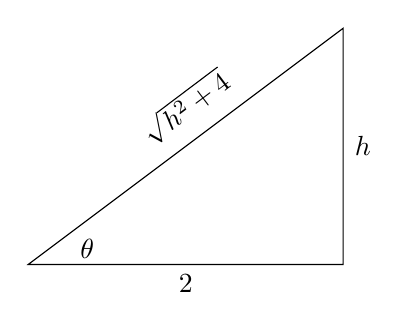
\begin{tikzpicture}
\draw (0,0)--(4,0)--(4,3)--cycle;
\draw (.75,.2) node{$\theta$};
\draw (2,0) node[below]{2};
\draw (4.25,1.5) node{$h$};
\draw (2,2) node[rotate=37]{$\sqrt{h^2+4}$};
\end{tikzpicture}\end{center}
Using the triangle, $\cos\theta = \dfrac{2}{\sqrt{h^2+4}}$, so
\begin{align*}
\diff{\theta}{t}&=\frac{1}{2}\left(\frac{2}{\sqrt{h^2+4}}\right)^2\cdot\diff{h}{t}\\
&=\left(\frac{2}{h^2+4}\right)\diff{h}{t}
\intertext{So, the quantities we need to know one minute after liftoff (that is, when $t = \dfrac{1}{60}$) are $h\left(\dfrac{1}{60}\right)$ and $\ds\diff{h}{t}\left(\frac{1}{60}\right)$. Recall $h(t)=61750t^2$.}
h\left(\frac{1}{60}\right)&=\frac{61750}{3600}=\frac{1235}{72}\\
\diff{h}{t}&=2(61750)t\\
\diff{h}{t}\left(\frac{1}{60}\right)&=\frac{2(61750)}{60}=\frac{6175}{3}
\intertext{Returning to the equation
$\ds\diff{\theta}{t}=\left(\dfrac{2}{h^2+4}\right)\ds\diff{h}{t}
$:}
\diff{\theta}{t}\left(\frac{1}{60}\right)&=\left(\frac{2}{\left(\frac{1235}{72}\right)^2+4}\right)\left(\frac{6175}{3}
\right)\approx 13.8~\frac{\mathrm{rad}}{\mathrm{hour}}\approx 0.0038~\frac{\mathrm{rad}}{\mathrm{sec}}
\end{align*}

\end{solution}



\begin{Mquestion}[1998H]
A high speed train is traveling at 2 km/min
along a straight track. The train is moving away from a movie camera which
is located 0.5 km from the track.
\begin{enumerate}[(a)]
\item\label{s3.2train1} How fast is the distance between the train and the camera
increasing when they are 1.3 km apart?
\item\label{s3.2train2}  Assuming that the camera is always pointed at the train,
how fast (in radians per min) is the camera rotating when the train and the
camera are 1.3 km apart?
\end{enumerate}
\end{Mquestion}
\begin{hint} Your picture should be a triangle.
\end{hint}
\begin{answer}
\eqref{s3.2train1} $\dfrac{24}{13}\approx 1.85$ km/min \qquad
\eqref{s3.2train2} about $.592$ radians/min
\end{answer}
\begin{solution}
\eqref{s3.2train1}
Let $x(t)$ be the distance of the train along the track at
time $t$, measured
from the point on the track nearest the camera. Let $z(t)$ be the distance
from the camera to the train at time $t$.

\begin{center}
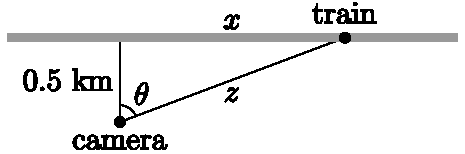
\includegraphics{train2}
\end{center}

Then \textcolor{red}{$x'(t)=2$} and at the time
in question, \textcolor{red}{$z(t)=1.3$} km and $\textcolor{red}{x(t)}=\sqrt{1.3^2-0.5^2}=\textcolor{red}{1.2}$ km. So
\begin{align*}
z(t)^2&=x(t)^2+0.5^2\\
 2z(t)z'(t)&=2x(t)x'(t)\\
 2\times 1.3z'(t)&=2\times 1.2\times 2\\
\color{red}z'(t)&\textcolor{red}{=\frac{2\times 1.2}{1.3}}\approx1.85 \mbox{ km/min}
\end{align*}

\eqref{s3.2train2}
Let $\theta(t)$ be the angle shown at time $t$. Then
\begin{align*}
\sin\left(\theta(t)\right)&=\frac{x(t)}{z(t)}\intertext{Differentiating with respect to $t$:}
\theta'(t)\cos\left(\theta(t)\right)
&=\frac{x'(t)z(t)-x(t)z'(t)}{z(t)^2}\\
\theta'(t)&=\frac{x'(t)z(t)-x(t)z'(t)}{z(t)^2\cos\left(\theta(t)\right)}
\intertext{From our diagram, we see $\cos\left(\theta(t)\right)=\dfrac{0.5}{z(t)}$, so:}
&=2\frac{x'(t)z(t)-x(t)z'(t)}{z(t)}
\intertext{Substituting in $x'(t)=2$, $z(t)=1.3$, $x(t)=1.2$, and $z'(t)=\dfrac{2\times1.2}{1.3}$:}
\theta'(t)
&=2\frac{2\times 1.3-1.2\times\frac{2\times 1.2}{1.3}}{1.3}
\approx .592  \mbox{ radians/min}
\end{align*}
\end{solution}


\begin{Mquestion}[1996D]
A ball is dropped from a height of $49$ metres above the ground. The
height of the ball at time $t$ is $h(t)=49-4.9 t^2$ m. A light, which is
also $49$ m above the ground, is $10$ m to the left of the ball's original
position. As the ball descends, the shadow of the ball caused by the light
moves across the ground. How fast is the shadow moving one second after
the ball is dropped?

\begin{center}
%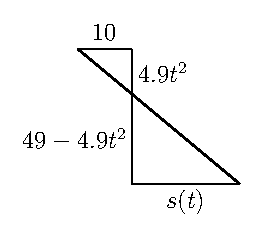
\includegraphics{ballShadow}
\begin{tikzpicture}
\draw[red, dashed] (0,3)--(6,0);
\draw[red] (0,3)--(2,3) node[midway, above]{10};
\draw[ultra thick] (0,0)--(0,3) node[midway, left]{49} node[opendot, label= left:{light}]{};
\draw[red, thick,<-] (2,1.5)--(2,3) ;
\draw[red, thick] (2,1.5)--(2,0) ;%node[above right]{ball};
\draw (2,2) node[shape=circle, minimum size=3mm, draw, fill=white, label=right:{$h(t)=49-4.9t^2$}]{};
\draw (1.75,2) node[left]{ball};
\draw[red] (2,0) -- (6,0) node[midway, below]{$s(t)$};
\end{tikzpicture}\end{center}
\end{Mquestion}
\begin{hint} In the diagram, find two similar triangles.
\end{hint}
\begin{answer} 200 m/s to the left
\end{answer}
\begin{solution}
In the diagram, there are two right triangles: one formed by the light, the ball, and the ball's original position, and one formed by the ball, the tip of its shadow, and the ball's eventual position on the ground. The two angles marked below have the same measure, $\alpha$. (Whenever two straight lines cross, the opposite angles formed have the same measure.)

\begin{center}
\begin{tikzpicture}
\draw[red, dashed] (0,3)--(6,0);
\draw[red] (0,3)--(2,3) node[midway, above]{10};
\draw[dashed, <->, thick](0,0)--(0,2) node[midway,left]{$49-4.9t^2$};
\draw[dashed, <->, thick](-1,2)--(-1,3) node[midway,left]{$4.9t^2$};
\draw[red, thick] (2,0)--(2,3) ;
\draw[red] (2,0) -- (6,0) node[midway, below]{$s(t)$};
\draw (2,2.25) node[above left]{$\alpha$};
\draw (2,1.75) node[below right]{$\alpha$};
\draw (2,2.25) arc(90:145:.25);
\draw (2,1.75) arc(-90:-35:.25);
\end{tikzpicture}\end{center}

Since the two triangles share two angles in common (a right angle, and an angle of measure $\alpha$), they are similar triangles.
Let's call $s(t)$ the distance from the shadow to the point
on the ground directly underneath the ball. Since the triangles are similar,
\begin{align*}
\frac{4.9 t^2}{10}&=\frac{49-4.9 t^2}{s(t)}\\
 s(t)&=10\frac{49-4.9 t^2}{4.9 t^2}=\frac{100}{t^2}-10\\
 s'(t)&=-2\frac{100}{t^3}
\end{align*}
When $t=1$, $s'(1)=-200$ m/sec. That is, {the shadow is moving to the
left at $200$ m/sec.}
\end{solution}

\begin{question}\label{s3.2triangleslast}
A clock has a minute hand that is 10 cm long, and an hour hand that is 5 cm long.
Let $D$ be the distance between the tips of the two hands. How fast is $D$ decreasing at 4:00?
\begin{center}\begin{tikzpicture}
\draw[ultra thick] node[shape=circle, minimum size=5cm, draw]{};
\draw node[vertex]{};
\draw[very thick, ->] (0,0)--(0,2) node(m){};
\draw[very thick, ->] (0,0)--(0.866,-.5) node(h){};
\draw[dashed, thick, red] (m)--(h) node[midway, right]{$D$};
\foreach \x in {0,...,11}{
	\draw (0,0)+(30*\x:2.1cm) node(o\x){};
	\draw (0,0)+(30*\x:2.75cm) node(i\x){};
	\draw (o\x)--(i\x);}
\end{tikzpicture}\end{center}
\end{question}
\begin{hint}
Let $\theta$ be the angle between the two hands. Using the Law of Cosines, you can get an expression for $D$ in terms of $\theta$.  To find $\ds\diff{\theta}{t}$, use what you know about how fast clock hands move.
\end{hint}
\begin{answer}
$\dfrac{55\sqrt{21}\pi}{42}\approx 19$ centimetres per hour.
\end{answer}
\begin{solution}
Let $\theta$ be the angle between the two hands.
\begin{center}\begin{tikzpicture}
\draw[ultra thick] node[shape=circle, minimum size=5cm, draw]{};
\draw node[vertex]{};
\draw[very thick, ->] (0,0)--(0,2) node(m){};
\draw[very thick, ->] (0,0)--(0.866,-.5) node(h){};
\draw[dashed, thick, red] (m)--(h) node[midway, right]{$D$};
\draw[red] (.25,.25) node{$\theta$};
\draw (.25,-.5) node[rotate=-30]{5cm};
\draw (-.35,1) node[rotate=90]{10cm};
\end{tikzpicture}\end{center}
The Law of Cosines (Appendix~\ref*{app cosine law}%B.4.11
) tells us that
\begin{align*}
D^2&=5^2+10^2-2\cdot5\cdot10\cdot\cos\theta\\
D^2&=125-100\cos\theta\intertext{Differentiating with respect to time $t$,}
2D\diff{D}{t}&=100\sin\theta\cdot\diff{\theta}{t}\\
\end{align*}
Our tasks now are to find  $D$, $\theta$ and $\ds\diff{\theta}{t}$ when the time is 4:00.
At 4:00, the minute hand is straight up, and the hour hand is $\dfrac{4}{12}=\dfrac{1}{3}$ of the way around the clock, so \textcolor{red}{$\theta = \dfrac{1}{3}(2\pi)=\dfrac{2\pi}{3}$} at 4:00. Then
$D^2=125-100\cos\left(\frac{2\pi}{3}\right)=125-100\left(-\frac{1}{2}\right)=175$, so
\textcolor{red}{$D=\sqrt{175}=5\sqrt{7}$} at 4:00.

To calculate $\ds\diff{\theta}{t}$, remember that both hands are moving. The hour hand makes a full rotation every 12 hours, so its rotational speed is $\dfrac{2\pi}{12}=\dfrac{\pi}{6}$ radians per hour. The hour hand is being chased by the minute hand. The minute hand makes a full rotation every hour, so its rotational speed is $\dfrac{2\pi}{1}=2\pi$ radians per hour. Therefore, the angle $\theta$ \emph{between} the two hands is changing at a rate of
\[\color{red}\ds\diff{\theta}{t}=-\left(2\pi-\dfrac{\pi}{6}\right)=\dfrac{-11\pi}{6}~~\frac{\mathrm{rad}}{\mathrm{hr}}.\]

Now, we plug in $D$, $\theta$, and $\ds\diff{\theta}{t}$ to find $\ds\diff{D}{t}$:
\begin{align*}
2D\diff{D}{t}&=100\sin\theta\cdot\diff{\theta}{t}\\
2\left(5\sqrt{7}\right)\diff{D}{t}&=100\sin\left(\frac{2\pi}{3}\right)\left(\frac{-11\pi}{6}\right)\\
10\sqrt{7}\diff{D}{t}&=
100\left(\frac{\sqrt3}{2}\right)\left(\frac{-11\pi}{6}\right)
=-\frac{275\pi}{\sqrt3}\\
\diff{D}{t}&=\frac{-55\sqrt{21}\pi}{42}  ~~\frac{\mathrm{cm}}{\mathrm{hr}}
\end{align*}
So $D$ is decreasing at $\dfrac{55\sqrt{21}\pi}{42} \approx 19$ centimetres per hour. \end{solution}


%%%%%%%%%%%%%%%%%%
%\subsubsection*{Problems that use formulas for volume or area}
%%%%%%%%%%%%%%%%%%
\Instructions{For Questions \ref{s3.2annulus} through \ref{s3.2formulaslast}, you'll need to know formulas for volume or area.}

\begin{question}[2006H]\label{s3.2annulus}
Find the rate of change of the area of the annulus
$\{ (x, y)~:~ r^2 \le x^2 + y^2 \le R^2 \}$.
(i.e. the points inside the circle of radius $R$ but outside the circle
of radius $r$) if \\$R = 3 ~\mathrm{cm}$, $r = 1~\mathrm{cm}$, $\ds\diff{R}{t} = 2~\frac{\mathrm{cm}}{\mathrm{s}}$, and $\ds\diff{r}{t} = 7~\frac{\mathrm{cm}}{\mathrm{s}}$.
\begin{center}\begin{tikzpicture}
\draw[thick] node[shape=circle, draw, minimum size=5cm, inner sep=0, fill=gray!20]{};
\draw[thick] node[shape=circle, draw, minimum size=2cm, inner sep=0, fill=white]{};
\draw node[vertex]{};
\draw (0,0)--(2.5,0) node[midway,above]{$R$};
\draw (0,-1)--(0,0) node[midway, left]{$r$};
\end{tikzpicture}\end{center}
\end{question}
\begin{hint}
The area in the annulus is the area of the outer circle minus the area of the inner circle.
\end{hint}
\begin{answer}
$\ds\diff{A}{t}=-2\pi~\dfrac{\mathrm{cm}^2}{\mathrm{s}}$
\end{answer}
\begin{solution}
The area at time $t$ is the area of the outer circle minus the area of the inner circle:\begin{align*}A(t)&=\pi\big(R(t)^2-r(t)^2\big)\\
\mbox{So, }~~A'(t)&=2\pi\big(R(t)R'(t)-r(t)r'(t)\big)
\intertext{Plugging in the given data,}
A'&=2\pi\big(3\cdot 2-1\cdot 7\big)=-2\pi
\end{align*}
So the area is \emph{shrinking} at a rate of $2\pi~\dfrac{\mathrm{cm}^2}{\mathrm{s}}$.
\end{solution}



\begin{question}
Two spheres are centred at the same point. The radius $R$ of the bigger sphere at time $t$ is given by $R(t)=10+2t$, while the radius $r$ of the smaller sphere is given by $r(t)=6t$, $t \ge 0$. How fast is the volume between the spheres (inside the big sphere and outside the small sphere) changing when the bigger sphere has a radius twice as large as the smaller?
\end{question}
\begin{hint}
The volume of a sphere with radius $R$ is $\dfrac{4}{3}\pi r^3$.
\end{hint}
\begin{answer}
$288$ cubic units per unit time
\end{answer}
\begin{solution}
The volume between the spheres, while the little one is inside the big one, is
\[V=\frac{4}{3}\pi R^3 - \frac{4}{3}\pi r^3\]
Differentiating implicitly with respect to $t$:
\[\diff{V}{t}=4\pi R^2\diff{R}{t}-4\pi r^2\diff{r}{t}\]

We differentiate $R=10+2t$ and $r=6t$ to find $\ds\diff{R}{t}=2$ and $\ds\diff{r}{t}=6$. When $R=2r$, $10+2t=2(6t)$, so $t=1$. When $t=1$, $R=12$ and $r=6$. So:
\[\diff{V}{t}=4\pi\left(12^2\right)(2)-4\pi\left(6^2\right)(6)=288\pi\]
So the volume between the two spheres is increasing at 288 cubic units per unit time.

Remark: when the radius of the inner sphere increases, we are ``subtracting" more area. Since the radius of the inner sphere grows faster than the radius of the outer sphere, we might expect the area between the spheres to be decreasing. Although the radius of the outer sphere grows more slowly, a small increase in the radius of the outer sphere results in a larger change in volume than the same increase in the radius of the inner sphere. So, a result showing that the volume between the spheres is increasing is not unreasonable.
\end{solution}



\begin{Mquestion}
You attach two sticks together at their ends, and stick the other ends in the mud. One stick is 150 cm long, and the other is 200 cm.
\begin{center}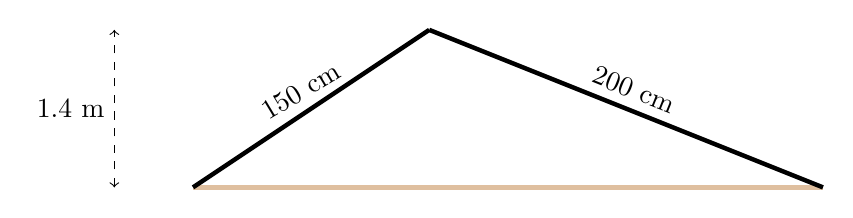
\begin{tikzpicture}
\draw[ultra thick, brown!50] (-3,0)--(5,0);
\draw[ultra thick] (-3,0)--(0,2)node[midway, above, rotate=31]{150 cm};
\draw[ultra thick] (0,2)--(5,0)node[midway, above, rotate=-22]{200 cm};
\draw[dashed, <->] (-4,0)--(-4,2) node[midway, left]{1.4 m};
\end{tikzpicture}\end{center}
The structure starts out being 1.4 metres high at its peak, but the sticks slide, and the height decreases at a constant rate of three centimetres per minute. How quickly is the area of the triangle (formed by the two sticks and the level ground) changing when the height of the structure is 120 cm?
\end{Mquestion}
\begin{hint}
The area of a triangle is half its base times its height. To find the base, split the triangle into two right triangles.
\end{hint}
\begin{answer}
0 square centimetres per minute
\end{answer}
\begin{solution}
We know something about the rate of change of the  height $h$ of the triangle, and we want to know something about the rate of change of its area, $A$. A reasonable plan is to find an equation relating $A$ and $h$, and differentiate implicitly with respect to $t$.
The area of a triangle with height $h$ and base $b$ is
\begin{align*}
A&=\frac{1}{2}bh\intertext{Note, $b$ will change with time as well as $h$. So, differentiating with respect to time, $t$:}
\diff{A}{t}&=\frac{1}{2}\left(\diff{b}{t}\cdot h+b\cdot\diff{h}{t}\right)
\end{align*}
We are given $\diff{h}{t}$ and $h$, but those $b$'s are a mystery. We need to relate them to $h$. We can do this by breaking our triangle into  two right triangles and using the Pythagorean Theorem:

\begin{center}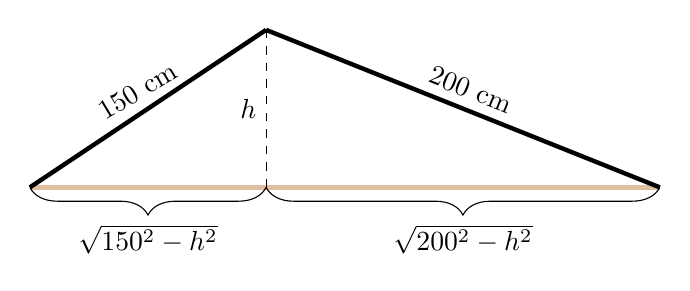
\begin{tikzpicture}
\draw[ultra thick, brown!50] (-3,0)--(5,0);
\draw[ultra thick] (-3,0)--(0,2)node[midway, above, rotate=31]{150 cm};
\draw[ultra thick] (0,2)--(5,0)node[midway, above, rotate=-22]{200 cm};
\draw[dashed] (0,0)--(0,2) node[midway, left]{$h$};
\draw[decorate, decoration={brace, mirror, amplitude=10pt}] (-3,0)--(0,0) node[midway,below,yshift=-10pt]{$\sqrt{150^2-h^2}$};
\draw[decorate, decoration={brace, mirror, amplitude=10pt}] (0,0)--(5,0) node[midway,below,yshift=-10pt]{$\sqrt{200^2-h^2}$};
\end{tikzpicture}\end{center}

So, the base of the triangle is
\begin{align*}b&=\sqrt{150^2-h^2}+\sqrt{200^2-h^2}
\intertext{Differentiating with respect to $t$:}
\diff{b}{t}&=\frac{-2h\diff{h}{t}}{2\sqrt{150^2-h^2}}+
\frac{-2h\diff{h}{t}}{2\sqrt{200^2-h^2}}\\
&=\frac{-h\diff{h}{t}}{\sqrt{150^2-h^2}}+
\frac{-h\diff{h}{t}}{\sqrt{200^2-h^2}}\intertext{Using $\ds\diff{h}{t}=-3$ centimetres per minute:}
\diff{b}{t}&=\frac{3h}{\sqrt{150^2-h^2}}+
\frac{3h}{\sqrt{200^2-h^2}}
\intertext{When $h=120$, $\sqrt{150^2-h^2}=90$ and $\sqrt{200^2-h^2}=160$. So, at this moment in time:}
b&=90+160=250\\
\diff{b}{t}&=\frac{3(120)}{90}+\frac{3(120)}{160}
=
4+\frac{9}{4}=\frac{25}{4}
\intertext{We return to our equation relating the derivatives of $A$, $b$, and $h$.}
\diff{A}{t}&=\frac{1}{2}\left(\diff{b}{t}\cdot h + b \cdot \diff{h}{t}\right)
\intertext{When $h=120$ cm, $b=250$, $\ds\diff{h}{t}=-3$, and $\ds\diff{b}{t}=\dfrac{25}{4}$:}
\diff{A}{t}&=\frac{1}{2}\left(\frac{25}{4}(120)+250(-3)\right)\\
&=0
\end{align*}

Remark: What does it mean that $\left.\ds\diff{A}{t}\right|_{h=120}=0$? Certainly, as the height changes, the area changes as well. As the height sinks to 120 cm, the area is increasing, but after it sinks \emph{past} 120 cm, the area is \emph{decreasing}. So, at the instant when the height is exactly 120 cm, the area is neither increasing nor decreasing: it is at a local maximum. You'll learn more about this kind of problem in Section~\ref*{sec optimise}.
\end{solution}




\begin{question}\label{s3.2segment}
The circular lid of a salt shaker has radius 8. There is a cut-out to allow the salt to pour out of the lid, and a door that rotates around to cover the cut-out. The door is a quarter-circle of radius 7 cm. The cut-out has the shape of a quarter-annulus with outer radius 6 cm and inner radius 1 cm.
If the uncovered area of the cut-out is $A$ cm$^2$, then the salt flows out at $\frac{1}{5}A$ cm$^3$ per second.

\begin{center}
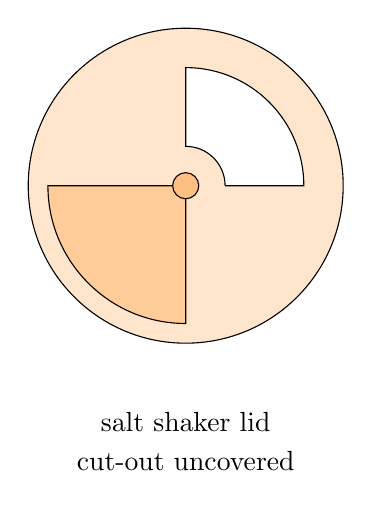
\begin{tikzpicture}
\draw node[shape=circle, minimum size=4cm, fill=orange!20,draw]{};
\draw[fill=white] (.5,0)--(1.5,0) arc(0:90:1.5cm)--(0,.5) arc(90:0:.5cm);
\draw[fill=orange!40] (0,0)--(0,-1.75) arc(-90:-180:1.75cm)--(0,0);
\draw[fill=orange!50] node[shape=circle, minimum size=1mm, draw, fill]{};
\draw (0,-3) node{salt shaker lid};
\draw (0,-3.5) node{cut-out uncovered};
\end{tikzpicture}\hspace{2cm}
%\begin{tikzpicture}
%\draw node[shape=circle, minimum size=4cm, fill=orange!20,draw]{};
%\draw[fill=white] (.5,0)--(1.5,0) arc(0:90:1.5cm)--(0,.5) arc(90:0:.5cm);
%\draw[fill=orange!40] (.5,0)--(1.5,0) arc(0:45:1.5cm)--(.35,.35) arc(45:0:.5cm);
%\draw[orange!75] node[shape=circle, minimum size=1mm, draw]{};
%\draw (0,-3) node{\textcolor{blue}{bottom} view of lid};
%\draw (0,-3.5) node{door half open: $\theta=\frac{\pi}{4}$};
%\end{tikzpicture}\hspace{2cm}
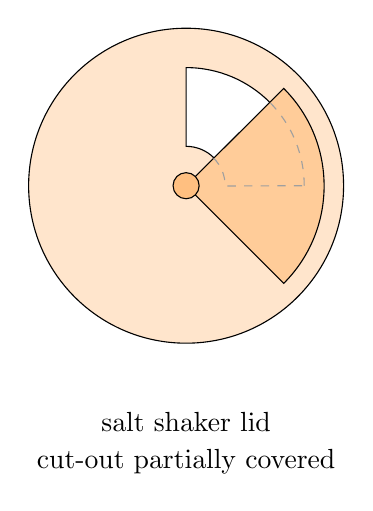
\begin{tikzpicture}
\draw node[shape=circle, minimum size=4cm, fill=orange!20,draw]{};
\draw[fill=white] (.5,0)--(1.5,0) arc(0:90:1.5cm)--(0,.5) arc(90:0:.5cm);
\draw[fill=orange!40] (0,0)--(1.24,-1.24) arc(-45:45:1.75cm)--(0,0);
\draw[fill=orange!50] node[shape=circle, minimum size=1mm, draw, fill]{};
\draw[dashed, gray!75] (1.5,0) arc(0:45:1.5cm) (.35,.35) arc(45:0:.5cm)--(1.5,0);
\draw (0,-3) node{salt shaker lid};
\draw (0,-3.5) node{cut-out partially covered};
\end{tikzpicture}
\end{center}
Recall: an annulus is the set of points inside one circle and outside another,  like a flat doughnut (see Question~\ref{s3.2annulus}).

\begin{center}
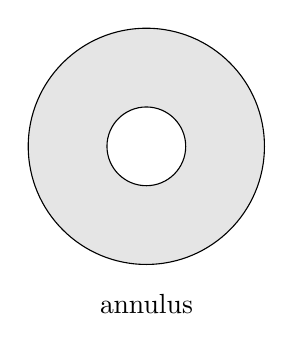
\begin{tikzpicture}
\draw (0,0) node[shape=circle, minimum size=3cm, draw, fill=gray!20]{};
\draw (0,0) node[shape=circle, minimum size=1cm, draw, fill=white]{};
\draw (0,-2) node{annulus};
\end{tikzpicture}
\hspace{2cm}
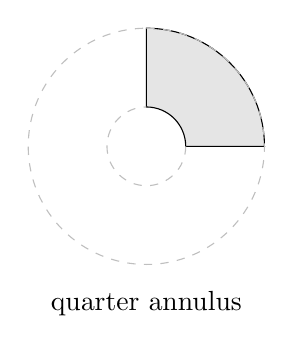
\begin{tikzpicture}
\draw[fill=gray!20] (.5,0) arc(0:90:.5cm)--(0,1.5) arc(90:0:1.5cm)--cycle;
\draw[gray!50, dashed] (.5,0) arc(0:-270:.5cm) (0,1.5) arc(90:-270:1.5cm);
\draw (0,-2) node{quarter annulus};
\end{tikzpicture}
\end{center}

While pouring out salt, you spin the door around the lid at a constant rate of $\frac{\pi}{6}$ radians per second, covering more and more of the cut-out. When exactly half of the cut-out is covered, how fast is the flow of salt changing?
\end{question}
\begin{hint}
The easiest way to figure out the area of the sector of an annulus (or a circle) is to
figure out the area of the entire annulus, then multiply by what proportion of the entire annulus the sector is. For example, if your sector is $\frac{1}{10}$ of the entire annulus, then its area is $\frac{1}{10}$ of the area of the entire annulus. (See Section~\ref*{app rad arc sec} %A.4
to  see how this works out for circles.)
\end{hint}
\begin{answer}
$-\dfrac{7\pi}{12}\approx -1.8~\dfrac{\mathrm{cm}^3}{\mathrm{sec}^2}$
\end{answer}
\begin{solution}
Let $S$ be the flow of salt (in cubic centimetres per second). We want to know $\ds\diff{S}{t}$: how fast the flow is changing at time $t$. We are given an equation for $S$:
\[S=\frac{1}{5}A\]
where $A$ is the uncovered area of the cut-out. So,
\[\diff{S}{t}=\frac{1}{5}\diff{A}{t}\]
If we can find $\ds\diff{A}{t}$, then we can find $\ds\diff{S}{t}$.
We are given information about how quickly the door is rotating. If we let $\theta$ be the angle made by the leading edge of the door and the far edge of the cut-out (shown below), then $\ds\diff{\theta}{t}=-\dfrac{\pi}{6}$ radians per second. (Since the door is covering more and more of the cut-out, $\theta$ is getting smaller, so $\ds\diff{\theta}{t}$ is negative.)

\begin{center}
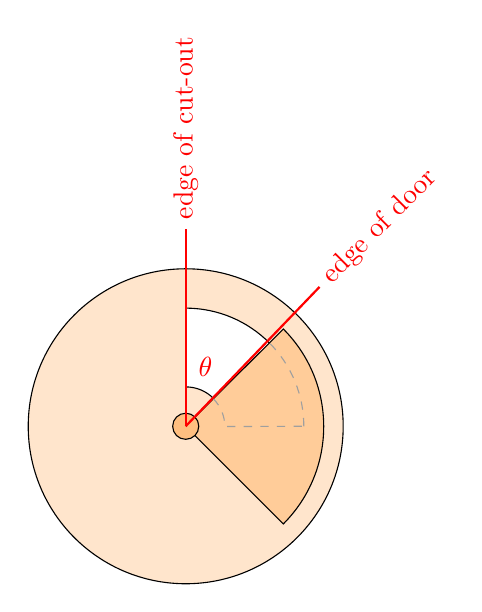
\begin{tikzpicture}
\draw node[shape=circle, minimum size=4cm, fill=orange!20,draw]{};
\draw[fill=white] (.5,0)--(1.5,0) arc(0:90:1.5cm)--(0,.5) arc(90:0:.5cm);
\draw[fill=orange!40] (0,0)--(1.24,-1.24) arc(-45:45:1.75cm)--(0,0);
\draw[fill=orange!50] node[shape=circle, minimum size=1mm, draw, fill]{};
\draw[dashed, gray!75] (1.5,0) arc(0:45:1.5cm) (.35,.35) arc(45:0:.5cm)--(1.5,0);
\draw[thick, red] (0,0)-- (0,2.5) node[right, rotate=90]{edge of cut-out};
\draw[thick, red] (0,0)--(1.7,1.77) node[right, rotate=45]{edge of door};
\draw[red] (.25,.75) node{$\theta$};
\end{tikzpicture}
\end{center}

Since we know $\ds\diff{\theta}{t}$, and we want to know $\ds\diff{A}{t}$ (in order to get $\ds\diff{S}{t}$), it is reasonable to look for an equation relating $A$ and $\theta$, and differentiate it implicitly with respect to $t$ to get an equation relating $\ds\diff{A}{t}$ and $\ds\diff{\theta}{t}$.

The area of an annulus with outer radius 6 cm and inner radius 1 cm is
$\pi\cdot 6^2-\pi\cdot1^2=35\pi$ square centimetres.
A sector of that same annulus with angle $\theta$ has area $\left(\frac{\theta}{2\pi}\right)(35\pi)$, since $\frac{\theta}{2\pi}$ is the ratio of the sector to the entire annulus. (For example, if $\theta=\pi$, then the sector is  \emph{half} of the entire annulus, so its area is $(1/2)35\pi$.)

So, when $0 \leq \theta \leq \frac{\pi}{2}$, the area of the cutout that is open is
\begin{align*}
A&=\frac{\theta}{2\pi}(35\pi)=\frac{35}{2}\theta
\intertext{This is the formula we wanted, relating $A$ and $\theta$. Differentiating with respect to $t$,}
\diff{A}{t}&=\frac{35}{2}\diff{\theta}{t}=\frac{35}{2}\left(-\frac{\pi}{6}\right)=-\frac{35\pi}{12}
\intertext{Since $\ds\diff{S}{t}=\frac{1}{5}\ds\diff{A}{t}$,}
\diff{S}{t}&=-\frac{1}{5}\frac{35\pi}{12}=-\frac{7\pi}{12}\approx -1.8~\frac{\mathrm{cm}^3}{\mathrm{sec}^2}
\end{align*}

Remark: the change in flow of salt is constant while the door covers more and more of the cut-out, so we never used the fact that precisely half of the cut-out was open. We also never used the radius of the lid, which is immaterial to the flow of salt.
\end{solution}


\begin{Mquestion}
A cylindrical sewer pipe with radius 1 metre has a vertical rectangular door that slides  in front of it to block the flow of water, as shown below. If the uncovered area of the pipe is $A$ m$^2$, then the flow of water through the pipe is $\frac{1}{5}A$ cubic metres per second.

The door slides over the pipe, moving vertically at a rate of 1 centimetre per second. How fast is the flow of water changing when the door covers the top 25 centimetres of the pipe?

\begin{center}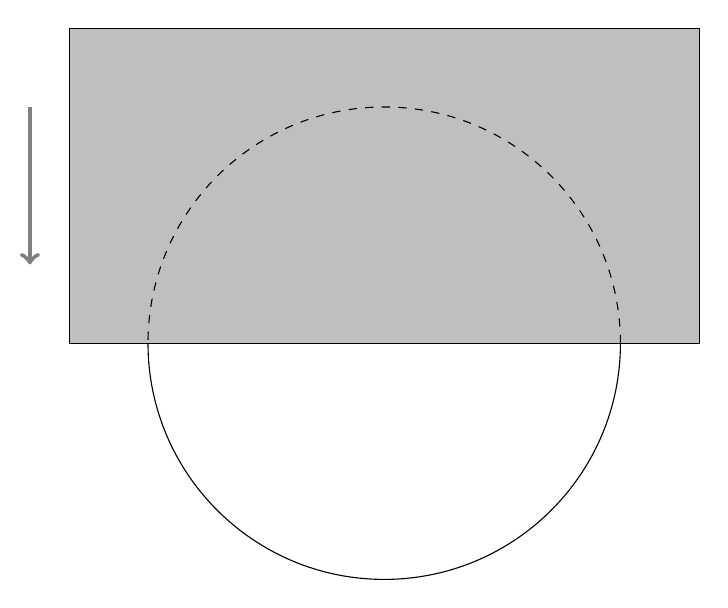
\begin{tikzpicture}
\draw (-3,0) arc(180:360:3cm);
\draw[fill=gray!50] (-4,0) rectangle (4,4);
\draw[dashed] (3,0) arc(0:180:3cm);
\draw[->, ultra thick, gray] (-4.5,3)--(-4.5,1);
\end{tikzpicture}\end{center}
\end{Mquestion}
\begin{hint}
Think about the ways in which this problem is similar to and different from
Example~\ref*{eg:fuel}
and Question~\ref{s3.2segment}.
\end{hint}
\begin{answer}
The flow is decreasing at a rate of $\dfrac{\sqrt{7}}{1000}~\dfrac{\mathrm{m}^3}{\mathrm{sec}^2}$.
\end{answer}
\begin{solution}
Let $F$ be the flow of water through the pipe, so $F=\dfrac{1}{5}A$. We want to know $\ds\diff{F}{t}$, so differentiating implicitly with respect to $t$, we find
\[\ds\diff{F}{t}=\frac{1}{5}\ds\diff{A}{t}.\]
If we can find $\ds\diff{A}{t}$, then we can find $\ds\diff{F}{t}$. We know something about the shape of the uncovered area of the pipe; a reasonable plan is to find an equation relating the height of the door with the uncovered area of the pipe. Let $h$ be the distance from the top of the pipe to the bottom of the door, measured in metres.

\begin{center}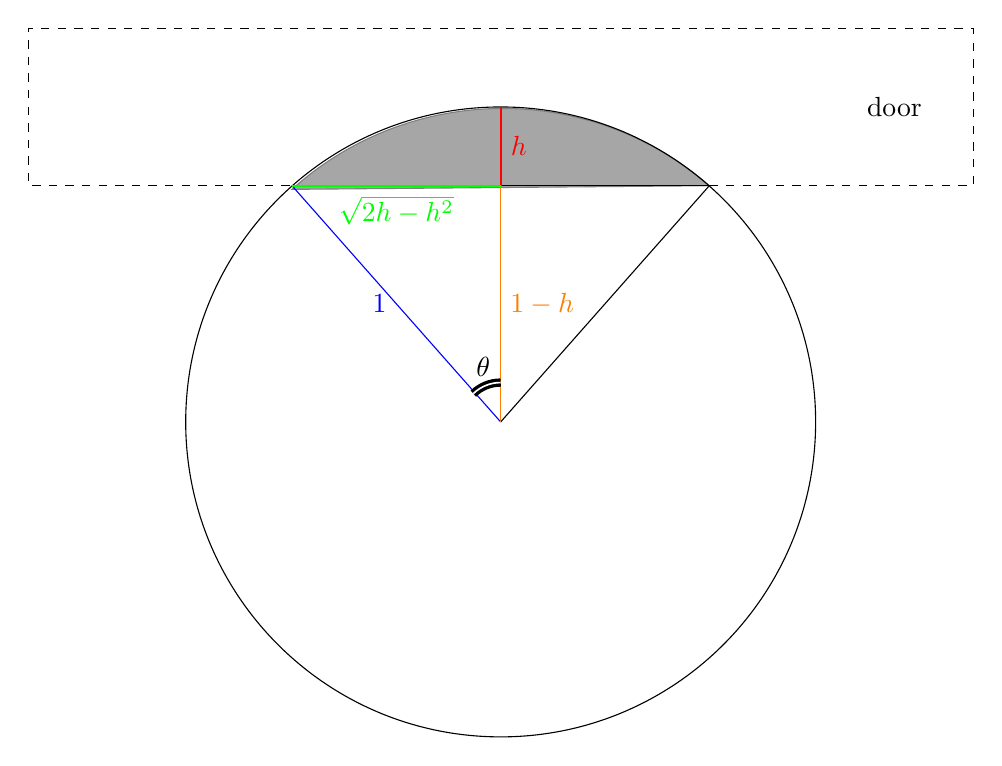
\begin{tikzpicture}
\draw[gray, fill=gray!70] (2.65,3) arc(49:132:4cm) --cycle;
\draw node[shape=circle, minimum size=8cm, draw]{};
\draw[dashed] (2.65,3)-|(6,5)-|(-6,3)--(-2.65,3);
\draw(-2.65,3)--(2.65,3);
\draw (5,4) node{door};
\draw[thick, red] (0,4)--(0,3) node[right, midway]{$h$};
\draw (0,0)--(2.65,3);
\draw[blue] (0,0)--(-2.65,3) node[left, midway]{1};
\draw[orange] (0,0)--(0,3) node[right, midway]{$1-h$};
\draw[thick, green] (-2.65,3)--(0,3) node[midway, below]{$\sqrt{2h-h^2}$};
%\draw[double, very thick] (0,.5) arc(90:134:.5) node[midway, above]{$\theta$};
\draw[double, very thick] (0,.5) arc(90:134:.5) ;
\draw (-0.22, 0.7) node{$\theta$};
\end{tikzpicture}\end{center}


Since the radius of the pipe is 1 metre, the orange line has length $1-h$ metres, and the blue line has length 1 metre. Using the Pythagorean Theorem, the green line has length $\sqrt{1^2-(1-h)^2}=\sqrt{2h-h^2}$ metres.

The uncovered area of the pipe can be broken up into a triangle (of height \textcolor{orange}{$1-h$} and base \textcolor{green}{$2\sqrt{2h-h^2}$}) and a sector of a circle (with angle $2\pi-2\theta$). The area of the triangle is \[\underbrace{(1-h)}_{\mbox{height}}\underbrace{\sqrt{2h-h^2}}_{\frac{1}{2}\mbox{base}}.\] The area of the sector is
\[\underbrace{\left(\frac{2\pi-2\theta}{2\pi}\right)}_{\atp{\mbox{fraction}}{\mbox{of circle}}}
\underbrace{(\pi\cdot 1^2)}_{
\atp{\mbox{area}
}{\mbox{of circle}
}}
=\pi-\theta.\]

Remember: what we want is to find $\ds\diff{A}{t}$, and what we know is
$\ds\diff{h}{t}=0.01$ metres per second.
If we find $\theta$ in terms of $h$, we find $A$ in terms of $h$, and then differentiate with respect to $t$.

Since $\theta$ is an angle in a right triangle with hypotenuse $1$ and adjacent side length $1-h$, $\cos\theta = \frac{1-h}{1} =1-h$. We want to conclude that $\theta = \arccos(1-h)$, but let's be a little careful: remember that the range of the arccosine function is angles in $[0,\pi]$. We must be confident that $0\le\theta\le\pi$ in order to conclude $\theta = \arccos(1-h)$--but clearly, $\theta$ is in this range. (Remark: we could also have said $\sin\theta=\frac{\sqrt{2h-h^2}}{1}$, and so $\theta = \arcsin\left(\sqrt{2h-h^2}\right)$. This would require $-\frac{\pi}{2}\leq \theta\leq\frac{\pi}{2}$, which is true when $h<1$, but false for $h>1$. Since our problem asks about $h=0.25$, we could also use arcsine.)

Now, we know the area of the open pipe in terms of $h$.
\begin{align*}
A&=(\mbox{area of triangle})+(\mbox{area of sector})\\
&=(1-h)\sqrt{2h-h^2}+(\pi-\theta)\\
&=(1-h)\sqrt{2h-h^2}+\pi-\arccos\left(1-h\right)
\intertext{We want to differentiate with respect to $t$. Using the chain rule:}
\diff{A}{t}&=\diff{A}{h}\cdot\diff{h}{t}\\
\diff{A}{t}&=\left((1-h)\frac{2-2h}{2\sqrt{2h-h^2}}+(-1)\sqrt{2h-h^2}
+\frac{-1}{\sqrt{1-(1-h)^2}}\right)\diff{h}{t}\\
&=\left(\frac{(1-h)^2}{\sqrt{2h-h^2}}-\sqrt{2h-h^2}-\frac{1}{\sqrt{2h-h^2}}\right)\diff{h}{t}\\
&=\left(\frac{(1-h)^2-1}{\sqrt{2h-h^2}}-\sqrt{2h-h^2}\right)\diff{h}{t}\\
&=\left(\frac{-(2h-h^2)}{\sqrt{2h-h^2}}-\sqrt{2h-h^2}\right)\diff{h}{t}\\
&=\left(-\sqrt{2h-h^2}-\sqrt{2h-h^2}\right)\diff{h}{t}\\
&=-2\sqrt{2h-h^2}\diff{h}{t}
\intertext{We note here that the negative sign makes sense: as the door lowers, $h$ increases and $A$ decreases, so $\ds\diff{h}{t}$ and $\ds\diff{A}{t}$ should have opposite signs.}
\intertext{When $h=\dfrac{1}{4}$ metres, and $\ds\diff{h}{t}=\frac{1}{100}$ metres per second:}
\diff{A}{t}&=-2\sqrt{\frac{2}{4}-\frac{1}{4^2}}\left(\frac{1}{100}\right)=-\frac{\sqrt{7}}{200}~\frac{\mathrm{cm}^2}{\mathrm{s}}
\intertext{Since $\ds\diff{F}{t}=\frac{1}{5}\ds\diff{A}{t}$:}
\diff{F}{t}&=-\frac{\sqrt{7}}{1000}~\frac{\mathrm{m}^3}{\mathrm{sec^2}}
\end{align*}
That is, the flow is decreasing at a rate of $\dfrac{\sqrt{7}}{1000}~\dfrac{\mathrm{m}^3}{\mathrm{sec}^2}$.
\end{solution}

\begin{Mquestion}\label{s3.2formulaslast}
A martini glass is shaped like a cone, with top diameter 10 cm and side length 10 cm.
\begin{center}\begin{tikzpicture}
\draw (0,0) node[ellipse, minimum width=6cm,draw]{};
\draw (-3,0)--(0,-5.2)--(3,0);
\draw[<->, gray] (-3,1)--(3,1);
\draw (0,1) node[shape=circle, fill=white, inner sep=0]{10};
\draw[<->, gray] (4,0)--(1,-5.2);
\draw (2.5,-2.6) node[shape=circle, fill=white, inner sep=0]{10};
\draw[<->, gray] (-4,0)--(-1,-5.2);
\draw(-2.5,-2.6) node[shape=circle, fill=white, inner sep=0]{10};
\end{tikzpicture}\end{center}
When the liquid in the glass is 7 cm high, it is evaporating at a rate of 5 mL per minute. How fast is the height of the liquid decreasing?
\end{Mquestion}
\begin{hint}
The volume of a cone with height $h$ and radius $r$ is $\frac{1}{3}\pi r^2h$.
Also, one millilitre is the same as one cubic centimetre.
\end{hint}
\begin{answer}
$\dfrac{-15}{49\pi}\approx -0.097$  cm per minute
\end{answer}
\begin{solution}
We are given the rate of change of the volume of liquid, and are asked for the rate of change of the height of the liquid. So, we need an equation relating volume and height.

The volume $V$ of a cone with height $h$ and radius $r$ is $\frac{1}{3}\pi r^2h$. Since we know $\ds\diff{V}{t}$, and want to know $\ds\diff{h}{t}$, we need to find a way to deal with the unwanted variable $r$. We can find $r$ in terms of $h$ by using similar triangles. Viewed from the side, the conical glass is an equilateral triangle, as is the water in it. Using the Pythagorean Theorem, the cone has height $5\sqrt{3}$.

\begin{center}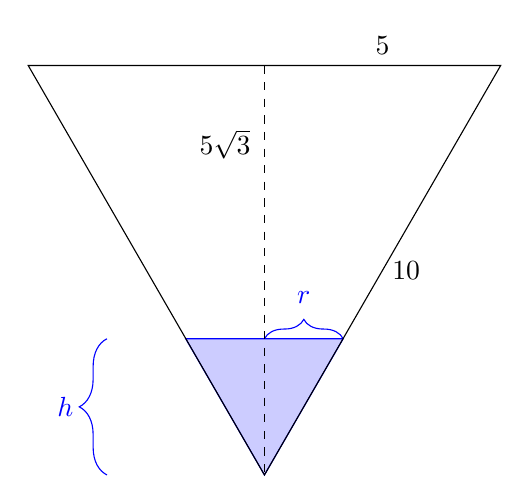
\begin{tikzpicture}
\color{blue}
\draw[fill=blue!20] (0,-5.2)--(1,-3.47)--(-1,-3.47)--cycle;
\draw[decorate, decoration={brace, amplitude=10pt}] (-2,-5.2)--(-2,-3.47) node
[midway, xshift=-15pt]{$h$};
\draw[decorate, decoration={brace, amplitude=7pt}] (0,-3.47)--(1,-3.47) node
[midway, yshift=15pt]{$r$};
\color{black}
\draw (-3,0)--(0,-5.2)--(3,0) node[midway, right]{10}--cycle;
\draw (1.5,.25) node{5};
\draw[dashed] (0,0)--(0,-5.2);
\draw (-.5,-1) node{$5\sqrt{3}$};
\end{tikzpicture}\end{center}

Using similar triangles, $\dfrac{r}{h}=\dfrac{5}{5\sqrt{3}}$, so $r=\dfrac{h}{\sqrt{3}}$. (Remark: we could also use the fact that the water forms a cone that looks like an equilateral triangle when viewed from the side to conclude $r=\dfrac{h}{\sqrt{3}}$.)

Now, we can write the volume of water in the cone in terms of $h$, and no other variables.
\begin{align*}
V&=\frac{1}{3}\pi r^2h\\
&=\frac{1}{3}\pi \left(\frac{h}{\sqrt{3}}\right)^2h\\
&=\frac{\pi}{9}h^3
\intertext{Differentiating with respect to $t$:}
\diff{V}{t}&=\frac{\pi}{3}h^2\diff{h}{t}
\intertext{When $h=7$ cm and $\ds\diff{V}{t}=-5$ mL per minute,}
-5&=\frac{\pi}{3}(49)\diff{h}{t}\\
\diff{h}{t}&=\frac{-15}{49\pi}\approx -0.097 \mbox{ cm per minute}
\end{align*}
\end{solution}




%%%%%%%%%%%%%%%%%%
\subsection*{\Application}
%%%%%%%%%%%%%%%%%%

\begin{Mquestion}
A floating buoy is anchored to the bottom of a river. As the river flows, the buoy is pulled in the direction of flow until its 2-metre rope is taught. A sensor at the anchor reads the angle $\theta$ between the rope and the riverbed, as shown in the diagram below. This data is used to measure the depth $D$ of water in the river, which depends on time.
\begin{center}
\begin{tikzpicture}
\draw[line width=2pt] (-3,0)--(5,0);
\draw (0,0) node[shape=circle, fill, minimum size=2mm]{};
\draw[ultra thick] (0,0)--(3,2) node[above,shape=circle, minimum size=5mm, fill=orange,draw]{};
\draw[blue, snake=saw, ultra thick] (-3,2)--(5,2);
\draw[very thick, ->, blue] (4,1.75)--(5,1.75);
\draw[thick, double] (1,0) arc (0:32:1);
\draw (1.25,.4)node{$\theta$};
\draw[blue, dashed, ultra thick, <->] (-2,.1)--(-2,1.925) node[midway, right]{$D$};
\end{tikzpicture}
\end{center}
\begin{enumerate}[(a)]
\item If $\theta = \dfrac{\pi}{4}$ and $\ds\diff{\theta}{t}=0.25~\frac{\mathrm{rad}}{\mathrm{hr}}$, how fast is the depth $D$ of the water changing?
\item A measurement shows $\ds\diff{\theta}{t}=0$, but $\ds\diff{D}{t}\neq0$. Under what circumstances does this occur?
\item A measurement shows $\ds\diff{\theta}{t}>0$, but $\ds\diff{D}{t}<0$. Under what circumstances does this occur?
\end{enumerate}
\end{Mquestion}
\begin{hint}
If you were to install the buoy, how would you choose the length of rope? For which values of $\theta$ do $\sin\theta$ and $\cos\theta$ have different signs? How would those values of $\theta$ look on the diagram?
\end{hint}
\begin{answer}
(a) $\ds\diff{D}{t}=\dfrac{1}{2\sqrt{2}}$ metres per hour\\
(b) The river is higher than 2 metres.\\
(c) The river's flow has reversed direction. (This can happen near an ocean at high tide.)
\end{answer}
\begin{solution}
As is so often the case, we use a right triangle in this problem to relate the quantities.
\begin{center}
\begin{tikzpicture}
\draw[line width=2pt] (-3,0)--(5,0);
\draw (0,0) node[shape=circle, fill, minimum size=2mm]{};
\draw[ultra thick] (0,0)--(3,2) node[above,shape=circle, minimum size=5mm, fill=orange,draw]{};
\draw (1.25,1.25) node{$2$};
\draw[blue, snake=saw, ultra thick] (-3,2)--(5,2);
\draw[very thick, ->, blue] (4,1.75)--(5,1.75);
%\draw[thick] (1,0) arc (0:32:1) node[midway, right]{$\theta$};
\draw[thick, double] (1,0) arc (0:32:1);
\draw (1.25,.4)node{$\theta$};
\draw[blue] (3,0)--(3,2) node[midway, right]{$D$};
\end{tikzpicture}\end{center}
\begin{align*}
\sin\theta&=\frac{D}{2}\\
D&=2\sin\theta\intertext{Using the chain rule, we differentiate both sides with respect to time, $t$.}
\diff{D}{t}&=2\cos\theta\cdot\diff{\theta}{t}
\intertext{So, if $\ds\diff{\theta}{t}=0.25$ radians per hour and $\theta = \dfrac{\pi}{4}$ radians, then}
(a)\qquad\diff{D}{t}&=2\cos\left(\frac{\pi}{4}\right)\cdot 0.25=2\left(\frac{1}{\sqrt{2}}\right)\frac{1}{4}=\frac{1}{2\sqrt{2}}~\mbox{metres per hour}.
\end{align*}

Setting aside part (b) for a moment, let's think about (c). If $\ds\diff{\theta}{t}$
and $\ds\diff{D}{t}$ have different signs, then because $\ds\diff{D}{t}=2\cos\theta\cdot\ds\diff{\theta}{t}$, that means $\cos\theta<0$. We have to have a nonnegative depth, so $D>0$ and $D=2\sin\theta$ implies $\sin \theta >0$. If $\sin\theta\ge0$ and $\cos \theta<0$, then $\theta\in(\pi/2,\pi]$. On the diagram, that looks like this:
\begin{center}
\begin{tikzpicture}
\draw[line width=2pt] (-5,0)--(5,0);
\draw (0,0) node[shape=circle, fill, minimum size=2mm]{};
\draw[ultra thick] (0,0)--(-3,2) node[above,shape=circle, minimum size=5mm, fill=orange,draw]{};
\draw (-1.25,1.25) node{$2$};
\draw[blue, snake=saw, ultra thick] (-5,2)--(5,2);
\draw[very thick, ->, blue] (-4,1.75)--(-5,1.75);
%\draw[thick, double] (.75,0) arc (0:143:.75) node[midway, above]{$\theta$};
\draw[thick, double] (.75,0) arc (0:143:.75);
\draw (0.3,1.0) node{$\theta$};
\draw[blue] (-3,0)--(-3,2) node[midway, right]{$D$};
\end{tikzpicture}\end{center}
That is: the water has reversed direction. This happens, for instance, when a river empties into the ocean and the tide is high.  Skookumchuck Narrows provincial park, in the Sunshine Coast, has reversing rapids.

Now, let's return to (b). If the rope is only 2 metres long, and the river rises \emph{higher} than 2 metres, then our equation $D=2\sin\theta$ doesn't work any more: the buoy might be stationary underwater while the water rises or falls (but stays at or above $2$ metres deep).
\end{solution}



\begin{question}
A point is moving in the $xy$-plane along the quadrilateral shown below.
\begin{center}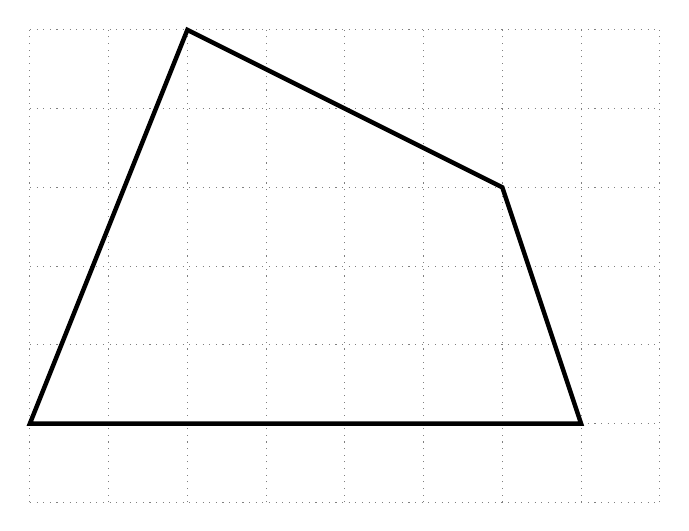
\begin{tikzpicture}
\YEaxis{4.25}{3.25}
\draw[dotted, gray] (-4,-3) grid (4,3);
\draw[ultra thick] (-2,3)--(-4,-2)--(3,-2)--(2,1)--cycle;
\YExcoord{1}{1}
\YEycoord{1}{1}
\end{tikzpicture}\end{center}
\begin{enumerate}[(a)]
\item When the point is at $(0,-2)$, it is moving to the right. An observer stationed at the origin must turn at a rate of one radian per second to keep looking directly at the point. How fast is the point moving?
\item When the point is at $(0,2)$, its $x$-coordinate is increasing at a rate of one unit per second. How fast it its $y$-coordinate changing? How fast is  the point moving?
\end{enumerate}
\end{question}
\begin{hint}
At both points of interest, the point is moving along  a straight line. From the diagram, you can figure out the equation of that line.

For the question ``How fast is the point moving?" in part (b), remember that the velocity of an object can be found by differentiating  (with respect to \emph{time}) the equation that gives the position of the object. The complicating factors in this case are that (1) the position of our object is not given as a function of time, and (2) the position of our object is given in two dimensions, not one.
\end{hint}
\begin{answer}
(a) 2 units per second
(b)
Its $y$-coordinate is decreasing at $\dfrac{1}{2}$ unit per second.\\
The point is moving at $\dfrac{\sqrt{5}}{2}$ units per second.
\end{answer}
\begin{solution}
(a) When the point is at $(0,-2)$, its $y$-coordinate is not changing, because it is moving along a horizontal line. So, the rate at which the particle moves is simply $\ds\diff{x}{t}$. Let $\theta$ be the angle an observer would be looking at, in order to watch the point.
Since we know $\ds\diff{\theta}{t}$, a reasonable plan is to find an equation relating $\theta$ and $x$, and then differentiate implicitly with respect to $t$. To do this, let's return to our diagram.

\begin{center}\begin{tikzpicture}
\YEaxis{4.25}{3.25}
\draw[ultra thick] (-2,3)--(-4,-2)--(3,-2)--(2,1)--cycle;
\draw (0,-2) node[vertex]{};
\draw (2,-2) node[vertex]{};
\draw[decorate, decoration={brace, amplitude=10pt}] (2,-2)--(0,-2) node[midway, yshift=-.6cm]{$x$};
\draw[dashed] (0,-2)--(0,0)--(2,-2);
\draw (.25,-.5) node{$\theta$};
\draw (-.25,-1) node{2};
\end{tikzpicture}\end{center}

When the point is a little to the right of $(0,-2)$, then we can make a triangle with the origin, as shown. If we let $\theta$ be the indicated angle, then $\ds\diff{\theta}{t}=1$ radian per second. (It is given that the observer is turning one radian per second, so this is how fast $\theta$ is increasing.) From the right triangle in the diagram, we see
\[\tan\theta=\frac{x}{2}\]
Now, we have to take care of a subtle point. The diagram we drew only makes sense for the point when it is at a position a little to the \emph{right} of $(0,-2)$. So, right now, we've only made a set-up that will find the derivative \emph{from the right}. But, with a little more thought, we see that even when $x$ is negative (that is, when the point is a little to the \emph{left} of $(0,-2)$), our equation holds if we are careful about how we define $\theta$. Let $\theta$ be  the angle between the line connecting the point and the origin, and the $y$-axis, where $\theta$ is \emph{negative} when the point is to the left of the $y$-axis.


\begin{center}\begin{tikzpicture}
\YEaxis{4.25}{3.25}
\draw[ultra thick] (-2,3)--(-4,-2)--(3,-2)--(2,1)--cycle;
\draw (0,-2) node[vertex]{};
\draw (-2,-2) node[vertex]{};
\draw[decorate, decoration={brace, amplitude=10pt, mirror}] (-2,-2)--(0,-2) node[midway, yshift=-.6cm]{$|x|$};
\draw[dashed] (0,-2)--(0,0)--(-2,-2);
%\draw (.25,-1) node{2};
\draw[decorate, decoration={brace, amplitude=10pt}] (0,0)--(0,-2) node[midway, xshift=.6cm]{$2$};
\draw[thick, double] (0,-.75)arc(270:225:.75cm);
\draw (-.4,-1) node{$|\theta|$};
\end{tikzpicture}\end{center}

Since $x$ and $\theta$ are both negative when the point is to the left of the $y$-axis,
\begin{align*}
\tan|\theta|&=\frac{2}{|x|}\\
\tan(-\theta) &= \frac{-x}{2}
\intertext{So, since $\tan(-\theta)=-\tan(\theta)$:}
\tan\theta&=\frac{x}{2}
\end{align*}
So, we've shown that the relationship $\tan\theta=\dfrac{x}{2}$ holds when our point is at $(x,-2)$, regardless of the sign of $x$.

Moving on, since we are given $\ds\diff{\theta}{t}$ and asked for $\ds\diff{x}{t}$, we differentiate with respect to $t$:
\begin{align*}
\sec^2\theta \cdot \diff{\theta}{t}&=\frac{1}{2}\cdot\diff{x}{t}
\intertext{When the point is at $(0,-2)$, since the observer is turning at one radian per second, also $\ds\diff{\theta}{t}=1$. Also, looking at the diagram, $\theta=0$. Plugging in these values:}
\sec^2\left(0\right)\cdot(1)&=\frac{1}{2}\cdot\diff{x}{t}\\
1&=\frac{1}{2}\cdot\diff{x}{t}\\
\diff{x}{t}&=2
\end{align*}
So, the particle is moving at 2 units per second.

(b) When the point is at $(0,2)$, it is moving along a line with slope $-\frac{1}{2}$ and $y$-intercept $2$. So, it is on the line
\[y=2-\frac{1}{2}x\]
That is, at time $t$, if the point is at $(x(t),y(t))$, then $x(t)$ and $y(t)$ satisfy
 $y(t)=2-\frac{1}{2}x(t)$. Implicitly differentiating with respect to $t$:
\[\diff{y}{t}=-\frac{1}{2}\cdot\diff{x}{t}\]
So, when $\ds\diff{x}{t}=1$, $\ds\diff{y}{t}=-\dfrac{1}{2}$. That is, its $y$-coordinate is decreasing at $\dfrac{1}{2}$ unit per second.

For the question ``How fast is the point moving?", remember that the velocity of an object can be found by differentiating  (with respect to \emph{time}) the equation that gives the position of the object. The complicating factors in this case are that (1) the position of our object is not given as a function of time, and (2) the position of our object is given in two dimensions (an $x$ coordinate and a $y$ coordinate), not one.

\textcolor{blue}{Remark: the solution below is actually pretty complicated.  It is within your abilities to figure it out, but later on in your mathematical career you will learn an easier way, using vectors. For now, take this as a relatively tough exercise, and a motivation to keep learning: your intuition that \emph{there must be an easier way} is well founded!}

The point is moving along a straight line. So, to take care of complication (2), we can give its position as a point on the line. We can take the line as a sort of axis. We'll need to choose a point on the axis to be the ``origin": $(2,1)$ is a convenient point. Let $D$ be the point's (signed) distance along the ``axis" from $(2,1)$. When the point is a distance of one unit to the left of $(2,1)$, we'll have $D=-1$, and
when the point is a distance of one unit to the right of $(2,1)$, we'll have $D=1$.
Then $D$ changes with respect to time, and $\ds\diff{D}{t}$ is the velocity of the point. Since we know $\ds\diff{x}{t}$ and $\ds\diff{y}{t}$, a reasonable plan is to find an equation relating $x$, $y$, and $D$, and differentiate implicitly with respect to $t$. (This implicit differentiation takes care of complication (1).) Using the Pythagorean Theorem:

\begin{align*}
D^2&=(x-2)^2+(y-1)^2
\intertext{Differentiating with respect to $t$:}
2D\cdot\diff{D}{t}&=2(x-2)\cdot\diff{x}{t}+2(y-1)\cdot\diff{y}{t}
\intertext{We plug in $x=0$, $y=2$, $\diff{x}{t}=1$, $\diff{y}{t}=-\frac{1}{2}$,
and $D=-\sqrt{(0-2)^2+(2-1)^2}=-\sqrt{5}$ (negative because the point is to the left of $(2,1)$):}
-2\sqrt{5}\cdot\diff{D}{t}&=2(-2)(1)+2(1)\left(-\frac{1}{2}\right)\\
\diff{D}{t}&=\frac{\sqrt{5}}{2}~\mbox{units per second}
\end{align*}
\end{solution}


\begin{question}
You have a cylindrical water bottle 20 cm high, filled with water. Its cross section is a circle of radius 5. You slowly smoosh the sides, so the cross section becomes an ellipse with major axis (widest part) $2a$ and minor axis (skinniest part) $2b$.

\begin{center}\begin{tikzpicture}
\draw node[shape=ellipse, minimum width=4cm, minimum height=3.5cm, draw]{};
\draw (-2,0)--(-2,-2) (2,0)--(2,-2);
\draw (0,0)--(2,0) node[above, midway]{$5$};
\draw (0,0)--(0,1.75) node[left, midway]{$5$};
\draw (2,-2)arc (0:-180:2cm and 1.75cm);
\draw (-2.5,-1) node{20};

\draw[ultra thick, red,->] (3,-1)--(5,-1);

\draw (9,0)node[shape=ellipse, minimum width=5cm, minimum height=2.5cm, draw]{};
\draw (6.5,0)--(6.5,-2) (11.5,0)--(11.5,-2);
\draw (9,0)--(11.5,0) node[above, midway]{$a$};
\draw (9,0)--(9,1.25) node[left, midway]{$b$};
\draw (11.5,-2)arc (0:-180:2.5cm and 1.25cm);
\draw (6.,-1) node{20};
\end{tikzpicture}\end{center}

After $t$ seconds of smooshing the bottle, $a=5+t$ cm. The perimeter of the cross section is unchanged as the bottle deforms. The perimeter of an ellipse is actually quite difficult to calculate, but we will use an approximation derived by Ramanujan and assume that the perimeter $p$ of our ellipse is
\[p \approx \pi\left[3(a+b)+\sqrt{(a+3b)(3a+b)}\right].\]
The area of an ellipse is $\pi a b$.
\begin{enumerate}[(a)]
\item Give an equation that relates $a$ and $b$ (and no other variables).
\item Give an expression for the volume of the bottle as it is being smooshed, in terms of $a$ and $b$ (and no other variables).
\item Suppose the bottle was full when its cross section was a circle. How fast is the water spilling out when $a$ is twice as big as $b$?
\end{enumerate}
\end{question}
\begin{hint}
(a) Since the perimeter of the cross section of the bottle does not change, $p$ (the perimeter of the ellipse) is the same as the perimeter of the circle of radius 5.\\
(b) The volume of the bottle will be the area of its cross section times its height. This is always the case when you have some two-dimensional shape, and turn it into a three-dimensional object by ``pulling" the shape straight up. (For example, you can think of a cylinder as a circle that has been ``pulled" straight up. To understand why this formula works, think about what is means to measure the area of a shape in square centimetres, and the volume of an object in cubic centimetres.) \\
(c) You can use what you know about $a$ and the formula from (a) to find $b$ and $\ds\diff{b}{t}$. Then use the formula from $(b)$.
\end{hint}
\begin{answer}
(a)  $10\pi=\pi\left[3(a+b)+\sqrt{(a+3b)(3a+b)}\right]$ or equivalently,
$10=3(a+b)+\sqrt{(a+3b)(3a+b)}
$\\
(b) $20\pi a b$\\
(c) The water is spilling out at about
36.64 cubic centimetres per second. The exact amount is
 $-\dfrac{200\pi}{9+\sqrt{35}}\left(1-2\left(\dfrac{3\sqrt{35}+11}{3\sqrt{35}+13}\right)\right)~\dfrac{\mathrm{cm}^3}{\mathrm{sec}}$.
\end{answer}
\begin{solution}
(a) Since the perimeter of the bottle is unchanged (you aren't stretching the plastic), it is always the same as the perimeter before it was smooshed, which is the circumference of a circle of radius 5, or $2\pi(5)=10\pi$. So, using our approximation for the perimeter of an ellipse,
\begin{align*}
10\pi&=\pi\left[3(a+b)+\sqrt{(a+3b)(3a+b)}\right]\\
10&=3(a+b)+\sqrt{(a+3b)(3a+b)}
\end{align*}

(b) The area of the base of the bottle is $\pi a b$
(see Section~\ref*{app sec areas}), and its height is 20 cm, so the volume of the bottle is
\[V=20\pi a b\]

(c) As you smoosh the bottle, its volume decreases, so the water spills out. (If it turns out that the volume is increasing, then no water is spilling out--but life experience suggests, and our calculations verify, that this is not the case.)
The water will spill out at a rate of $-\ds\diff{V}{t}$ cubic centimetres per second, where $V$ is the volume inside the bottle. We know something about $a$ and $\ds\diff{a}{t}$, so a reasonable plan is to differentiate the equation from (b) (relating $V$ and $a$) with respect to $t$.

Using the product rule, we differentiate the equation in (b) implicitly with respect to $t$ and get
\[\diff{V}{t}=20\pi\left(\diff{a}{t}b+a\diff{b}{t}\right)\]

So, we need to find the values of \textcolor{red}{$a$}, \textcolor{red}{$b$},
\textcolor{red}{$\ds\diff{a}{t}$}, and \textcolor{red}{$\ds\diff{b}{t}$} at the moment when $a=2b$.

The equation from (a) tells us $10=3(a+b)+\sqrt{(a+3b)(3a+b)}$. So, when $a=2b$,
\begin{align*}
10&=3(2b+b)+\sqrt{(2b+3b)(6b+b)}\\
10&=9b+\sqrt{(5b)(7b)}=b\left(9+\sqrt{35}\right)\\
\color{red}b&\color{red}=\frac{10}{9+\sqrt{35}}
\intertext{where we use the fact that $b$ is a positive number, so $\sqrt{b^2}=|b|=b$. }\intertext{Since $a=2b$,}
\color{red}a&\color{red}=\frac{20}{9+\sqrt{35}}
\intertext{Now we know $a$ and $b$ at the moment when $a=2b$. We still need to know $\ds\diff{a}{t}$ and $\ds\diff{b}{t}$ at that moment. Since $a=5+t$, always
\textcolor{red}{$\ds\diff{a}{t}=1$}. The equation from (a) relates $a$ and $b$, so differentiating both sides with respect to $t$ will give us an equation relating $\ds\diff{a}{t}$ and $\ds\diff{b}{t}$. When differentiating the portion with a square root, be careful not to forget the chain rule.}
0&=3\left(\diff{a}{t}+\diff{b}{t}\right)+\frac{\left(\diff{a}{t}+3\diff{b}{t}\right)(3a+b)+(a+3b)\left(3\diff{a}{t}+\diff{b}{t}\right)}{2\sqrt{(a+3b)(3a+b)}}
\intertext{Since $\ds\diff{a}{t}=1$:}
0&=3\left(1+\diff{b}{t}\right)+\frac{\left(1+3\diff{b}{t}\right)(3a+b)+(a+3b)\left(3+\diff{b}{t}\right)}{2\sqrt{(a+3b)(3a+b)}}
\intertext{At this point, we could plug in the values we know for $a$ and $b$ at the moment when $a=2b$. However, the algebra goes a little smoother if we start by plugging in $a=2b$:}
0&=3\left(1+\diff{b}{t}\right)+\frac{\left(1+3\diff{b}{t}\right)(7b)+(5b)\left(3+\diff{b}{t}\right)}{2\sqrt{(5b)(7b)}}\\
0&=3\left(1+\diff{b}{t}\right)+\frac{b\left(7+21\diff{b}{t}+15+5\diff{b}{t}\right)}{2b\sqrt{35}}\\
0&=3\left(1+\diff{b}{t}\right)+\frac{22+26\diff{b}{t}}{2\sqrt{35}}\\
0&=3+3\diff{b}{t}+\frac{11}{\sqrt{35}}+\frac{13}{\sqrt{35}}\diff{b}{t}\\
-3-\frac{11}{\sqrt{35}}&=\left(3+\frac{13}{\sqrt{35}}\right)\diff{b}{t}\\
\color{red}\diff{b}{t}&=\frac{-3-\frac{11}{\sqrt{35}}}{3+\frac{13}{\sqrt{35}}}=\color{red}\frac{-3\sqrt{35}-11}{3\sqrt{35}+13}
\intertext{Now, we can calculate $\ds\diff{V}{t}$ at the moment when $a=2b$. We already found}
\diff{V}{t}&=20\pi\left(\diff{a}{t}b+a\diff{b}{t}\right)
\intertext{So, plugging in the values of $a$, $b$, $\ds\diff{a}{t}$, and $\ds\diff{b}{t}$ at the moment when $a=2b$:}
\diff{V}{t}&=20\pi\left((1)\left(\frac{10}{9+\sqrt{35}}\right)+\left(\frac{20}{9+\sqrt{35}}\right)\left(\frac{-3\sqrt{35}-11}{3\sqrt{35}+13}\right)\right)\\
&=\frac{200\pi}{9+\sqrt{35}}\left(1-2\left(\frac{3\sqrt{35}+11}{3\sqrt{35}+13}\right)\right)\\
&\approx -36.64~\frac{\mathrm{cm}^3}{\mathrm{sec}}
\end{align*}
So the water is spilling out of the cup at about 36.64 cubic centimetres per second.

Remark: the algebra in this problem got a little nasty, but the method behind its solution is no more difficult than most of the problems in this section. One of the reasons why calculus is so widely taught in universities is to give you lots of practice with problem-solving: taking a big problem, breaking it into pieces you can manage, solving the pieces, and getting a solution.

A problem like this can sometimes derail people. Breaking it up into pieces isn't so hard, but when you actually do those pieces, you can get confused and forget why you are doing the calculations you're doing. If you find yourself in this situation, look back a few steps to remind yourself why you started the calculation you just did. It can also be helpful to write notes, like
``We are trying to find $\diff{V}{t}$. We already know that
                $\diff{V}{t} = ...$. We still need to find $a$, $b$,
                $\diff{a}{t}$ and $\diff{b}{t}$."
                % ``need to know $a$, $b$, $\diff{a}{t}$, and $\diff{b}{t}$ for equation $\diff{V}{t}=20\pi\left(\diff{a}{t}b+a\diff{b}{t}\right)$."
\end{solution}



\begin{question}
The quantities $A$, $B$, $C$, and $D$ all depend on time, and are related by the formula
\[AB=\log\left(C^2+D^2+1\right).\]
At time $t=10$, the following values are known:
\begin{itemize}
\item $A=0$
\item $\ds\diff{A}{t}=2$ units per second
\end{itemize}
What is $B$ when $t=10$?
\end{question}
\begin{hint}
If $A=0$, you can figure out $C$ and $D$ from the relationship given.
\end{hint}
\begin{answer}
% $B(10)=\dfrac{1}{2}$
$B(10)=0$
\end{answer}
\begin{solution}
Since $A=0$, the equation relating the variables tells us:
\begin{align*}
0&=\log\left(C^2+D^2+1\right)\\
1&=C^2+D^2+1\\
0&=C^2+D^2\\
0&=C=D
\intertext{This will probably be useful information. Since we're also given the value of a derivative, let's differentiate the equation relating the variables implicitly with respect to $t$. For ease of notation, we will write $\ds\diff{A}{t}=A'$, etc.}
A'B+AB'&=\frac{2CC'+2DD'}{C^2+D^2+1}
\intertext{At $t=10$, $A=C=D=0$:}
A'B+0&=\frac{0+0}{0+0+1}\\
% A'B&=1
A'B&=0
\intertext{at $t=10$, $A'=2$ units per second:}
% 2B&=1\\
% B&=\frac{1}{2}
2B&=0\\
B&=0.
\end{align*}
\end{solution}
